\chapter{Results}\label{ch:results}
%**********************************************
\section{Current sensor} \label{sec:current_sense_results}
%**********************************************

\subsection{Simulation}

Figure \ref{fig:cursen_sim_res} shows the simulation results for the circuit shown in Figure: \ref{fig:cursen_sim_cir}. The requirement for a \SI{10}{\milli\volt} signal at \SI{1}{\kilo\hertz} to result in less than \SI{250}{\milli\volt} at the output, is shown to be met in \ref{subfig:cursen_sim_noise} where the \SI{10}{\milli\volt} signal at \SI{1}{\kilo\hertz} results in an output of $\approx$\SI{160}{\milli\volt}. Figure \ref{subfig:cursen_sim_step} shows that the circuit has a response time less than 100ms, with a response time of $\approx$\SI{30}{\milli\second}. The requirement that the amplification circuit draws less than \SI{150}{\micro\ampere} is met in Figure: \ref{subfig:cursen_sim_curdraw} where the maximum current draw is \SI{83}{\micro\ampere}.

\begin{figure}[H]
\centering
\begin{subfigure}[]{0.45\textwidth}
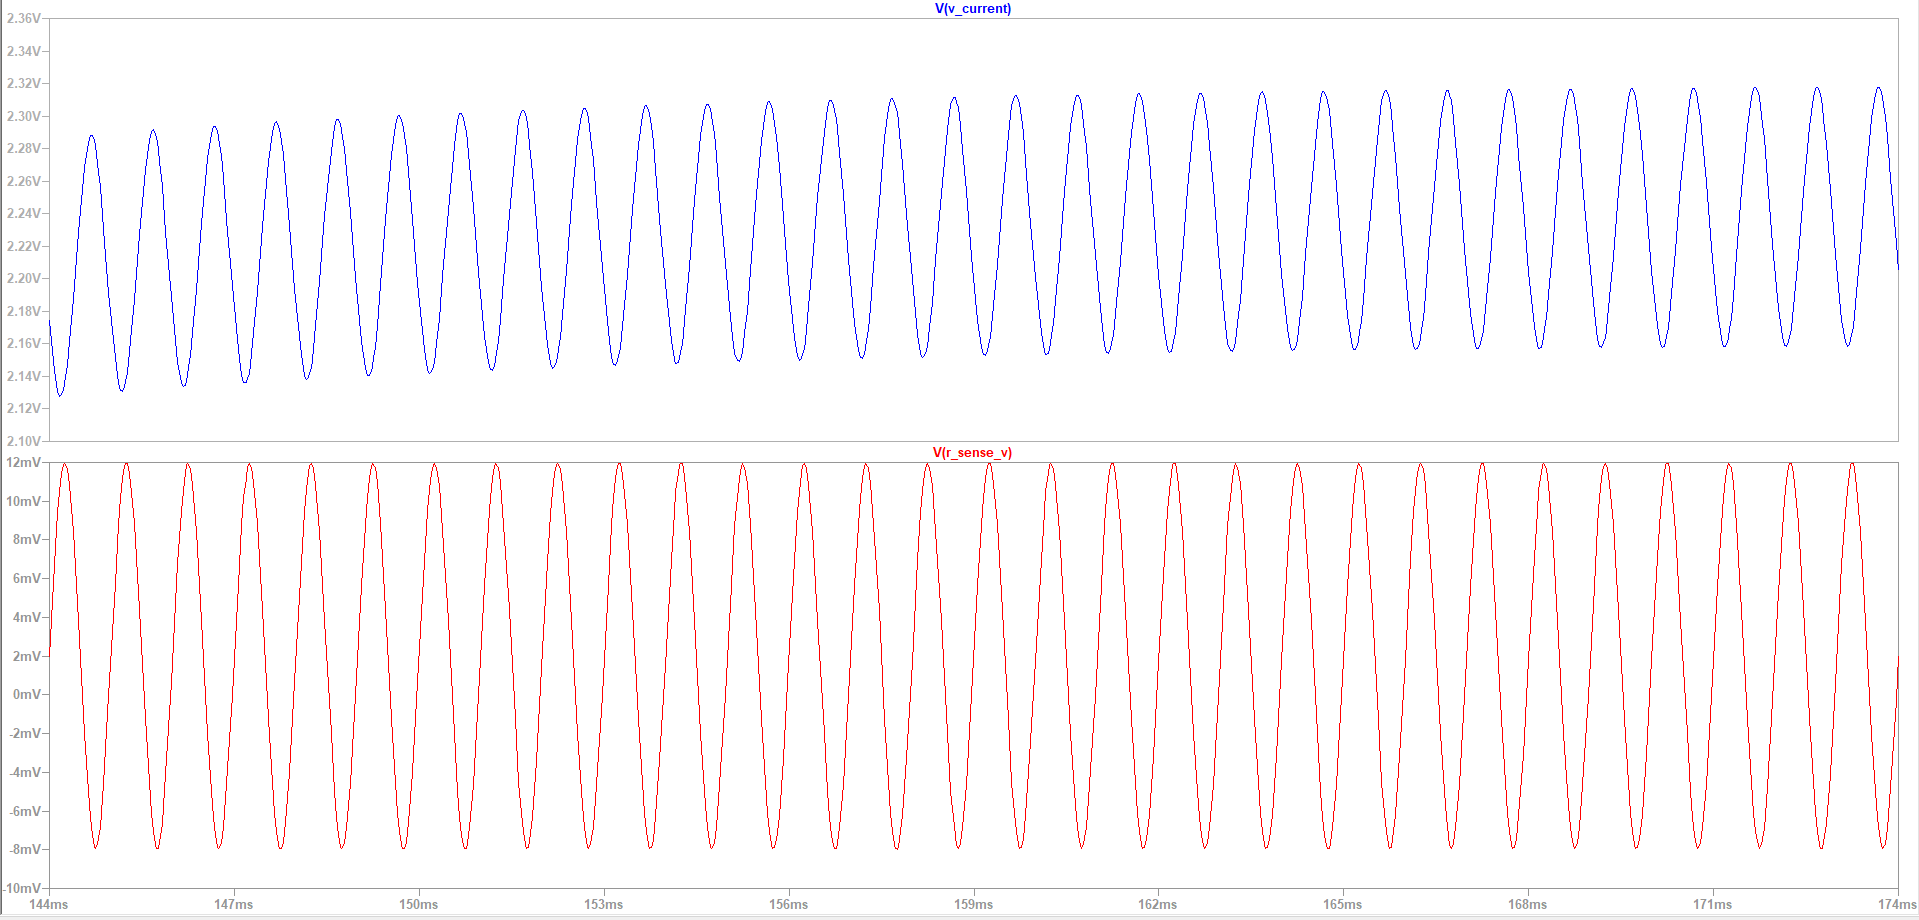
\includegraphics[width=\linewidth]{./Figures/CurSens_NoiseResp.png}
\caption{Noise input vs output of current sensing circuit.}
\label{subfig:cursen_sim_noise}	
\end{subfigure}
\hfill
\begin{subfigure}[]{0.45\textwidth}
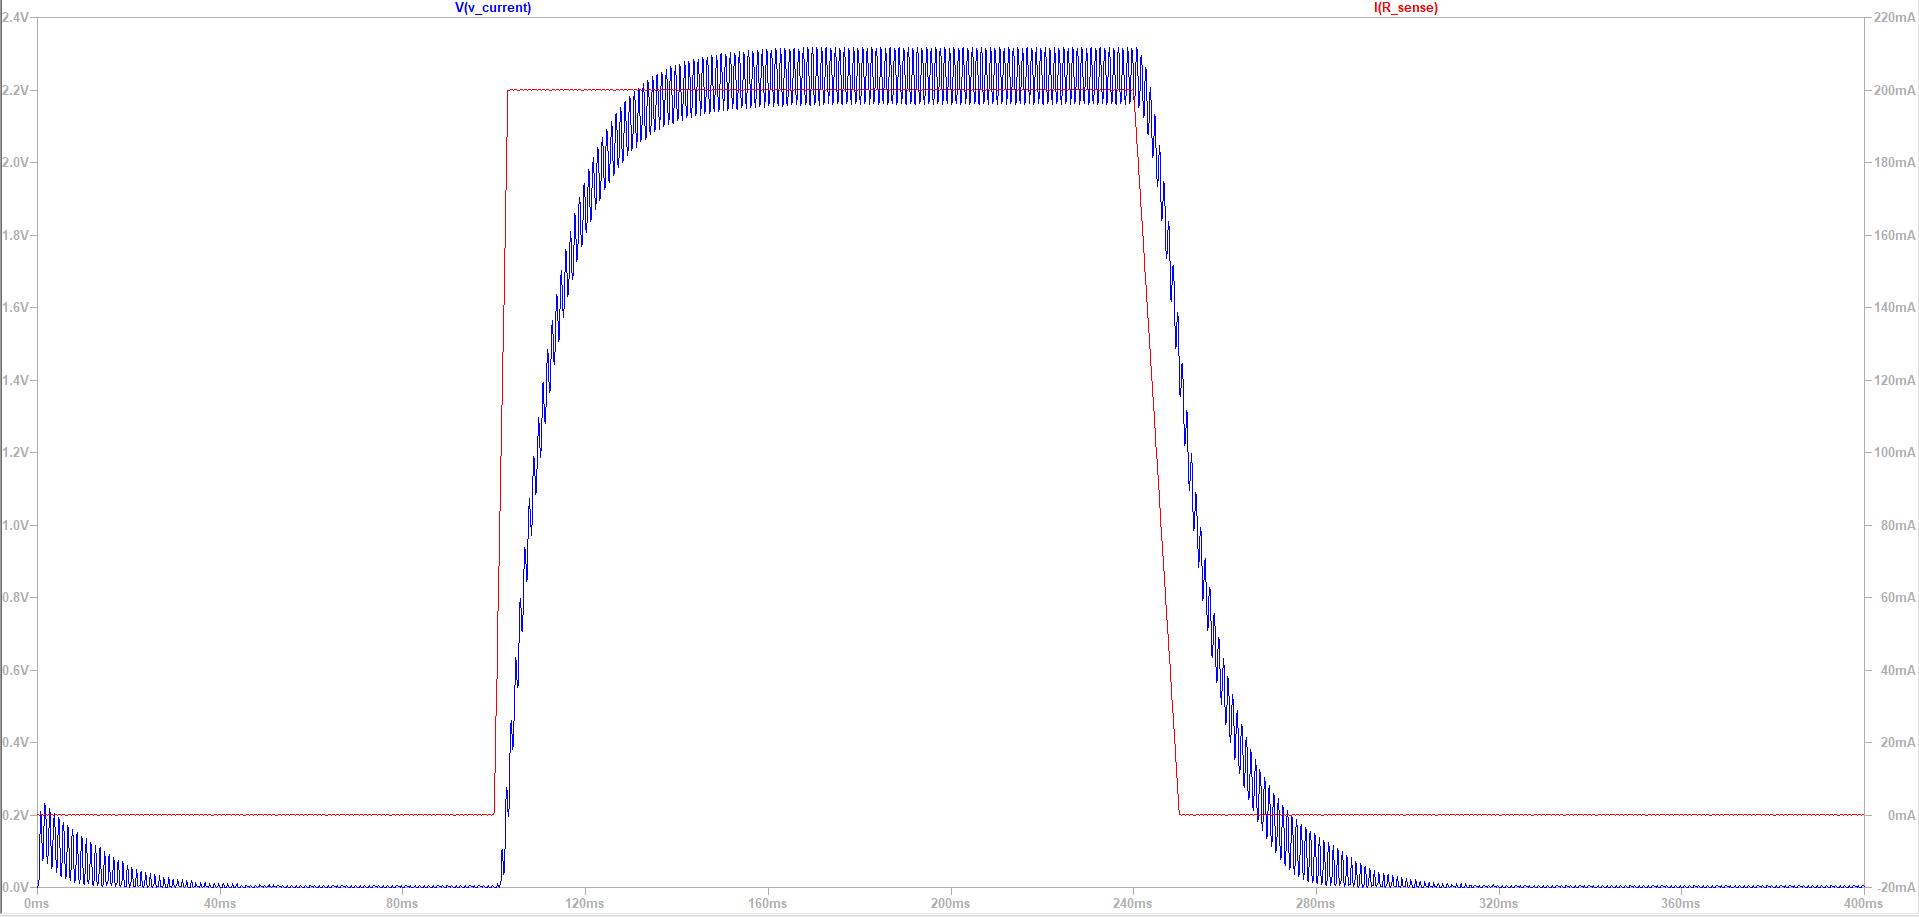
\includegraphics[width=\linewidth]{./Figures/CurSens_StepResp.png}
\caption{Step response of current sensing circuit.} 			
\label{subfig:cursen_sim_step}	
\end{subfigure}
\vspace{2pt}
\begin{subfigure}[]{0.45\textwidth}
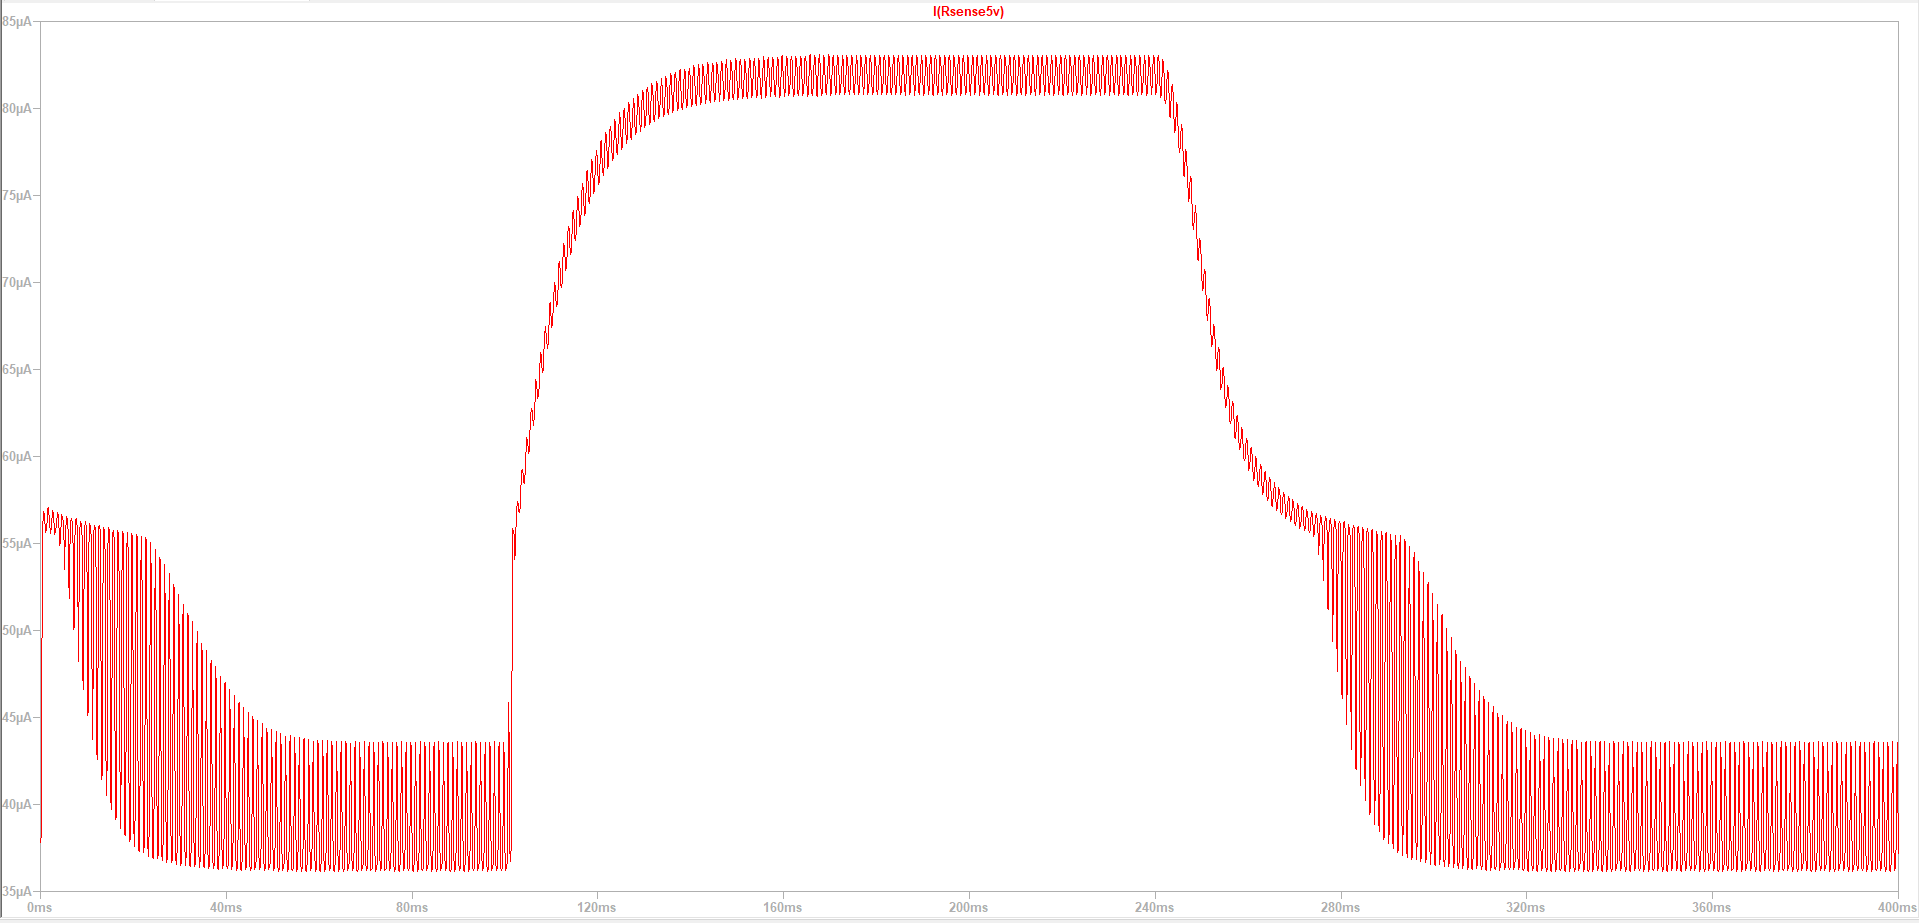
\includegraphics[width=\linewidth]{./Figures/CurSens_CurDraw.png}
\caption{Current draw of 5V supply to current sensing circuit.}
\label{subfig:cursen_sim_curdraw}	
\end{subfigure}
\caption{Current sensing circuit simulation results}
\label{fig:cursen_sim_res}
\end{figure}

\clearpage
\subsection{Practical}
As shown in Figure:\ref{fig:cursen_prac_resp} the practical results match the simulated results shown in Figure: \ref{fig:cursen_sim_res}. 

The practical response to no input (\ref{subfig:cursen_prac_noin}) shows an output of \SI{66}{\milli\volt}, this differs from the simulation output of \SI{0}{\volt} due to the non ideal nature of practical op amps and is due to the offset voltage between the input terminals.

Figure: \ref{subfig:cursen_sim_step} shows an output voltage of \SI{2.2}{\volt} to a \SI{200}{\milli\ampere} input while Figure: \ref{subfig:cursen_prac_slight} shows a \SI{1.82}{\volt} output to a  \SI{200}{\milli\ampere} input. This is due to the practical circuit having a reduced gain in comparison to the simulation. This was done to reduce the affect of the input offset voltage mentioned previously. 

Figure: \ref{subfig:cursen_prac_stall} shows the output clips sat \SI{3.28}{\volt} which is very close to the theoretical \SI{3.3}{\volt}. 

Figure: \ref{subfig:cursen_prac_noise} shows a lesser response to noise than the simulation, this is due to the noise input to the practical circuit is different to the simulated noise and at a higher frequency so the low pass filter attenuates it more heavily.

The measure response time in Figure: \ref{subfig:cursen_prac_step} is \SI{24}{\milli\second} which is very close to the response time measured in the simulation of \SI{30}{\milli\second}.


\begin{figure}[H]
\centering
\begin{subfigure}[]{0.3\textwidth}
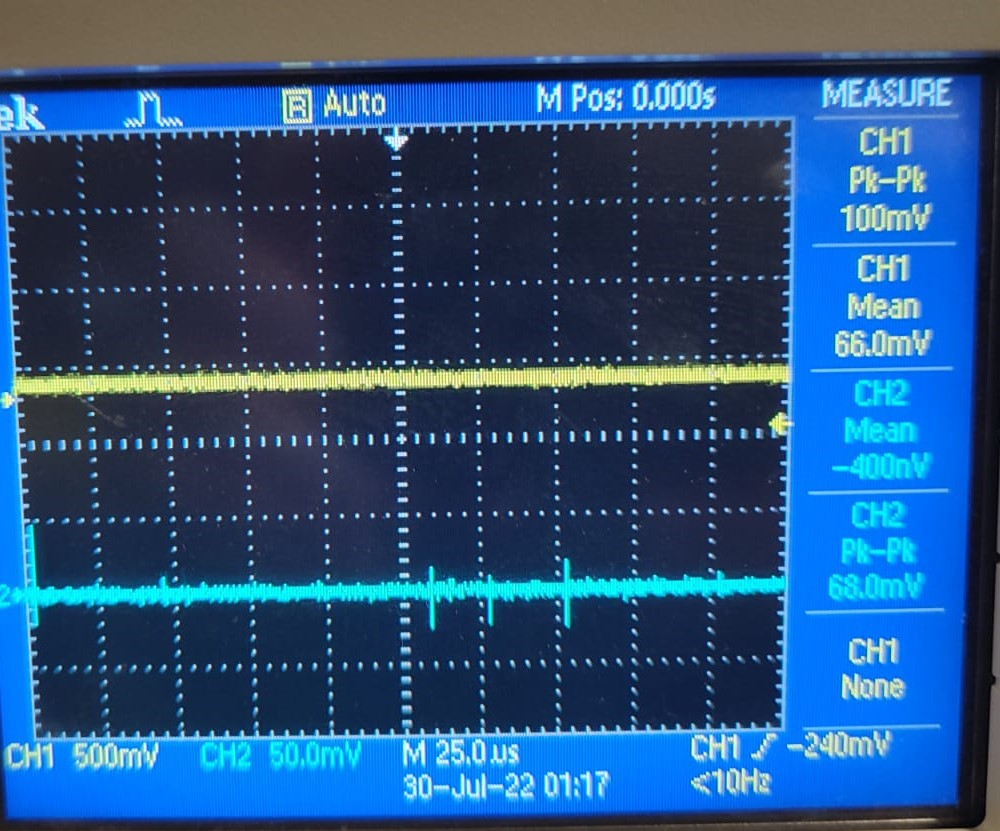
\includegraphics[width=\linewidth]{./Figures/CurSens_Prac_0input.jpeg}
\caption{Circuit response to no input.}
\label{subfig:cursen_prac_noin}	
\end{subfigure}
\hfill
\begin{subfigure}[]{0.3\textwidth}
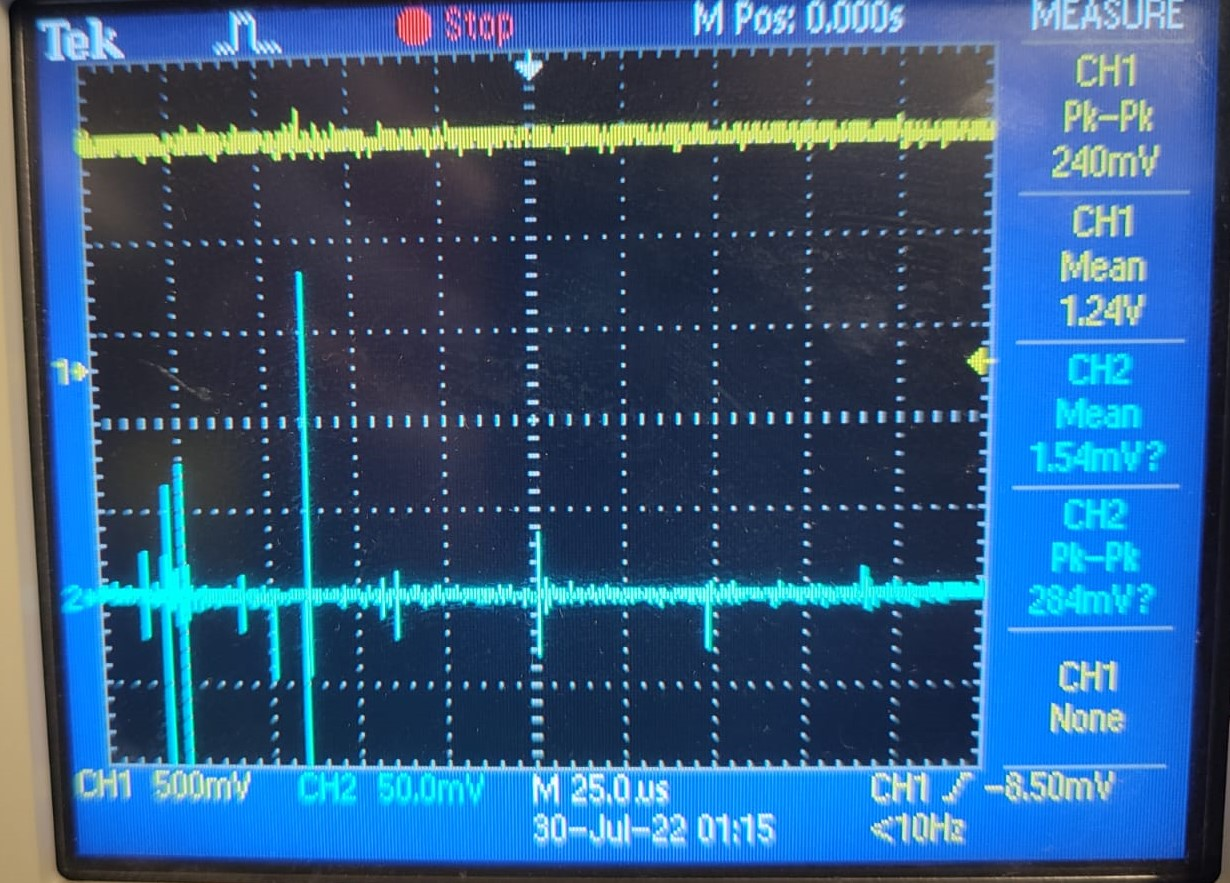
\includegraphics[width=\linewidth]{./Figures/CurSens_Prac_Free.jpeg}
\caption{Circuit response to free running motor.} 			
\label{subfig:cursen_prac_free}	
\end{subfigure}
\hfill
\begin{subfigure}[]{0.3\textwidth}
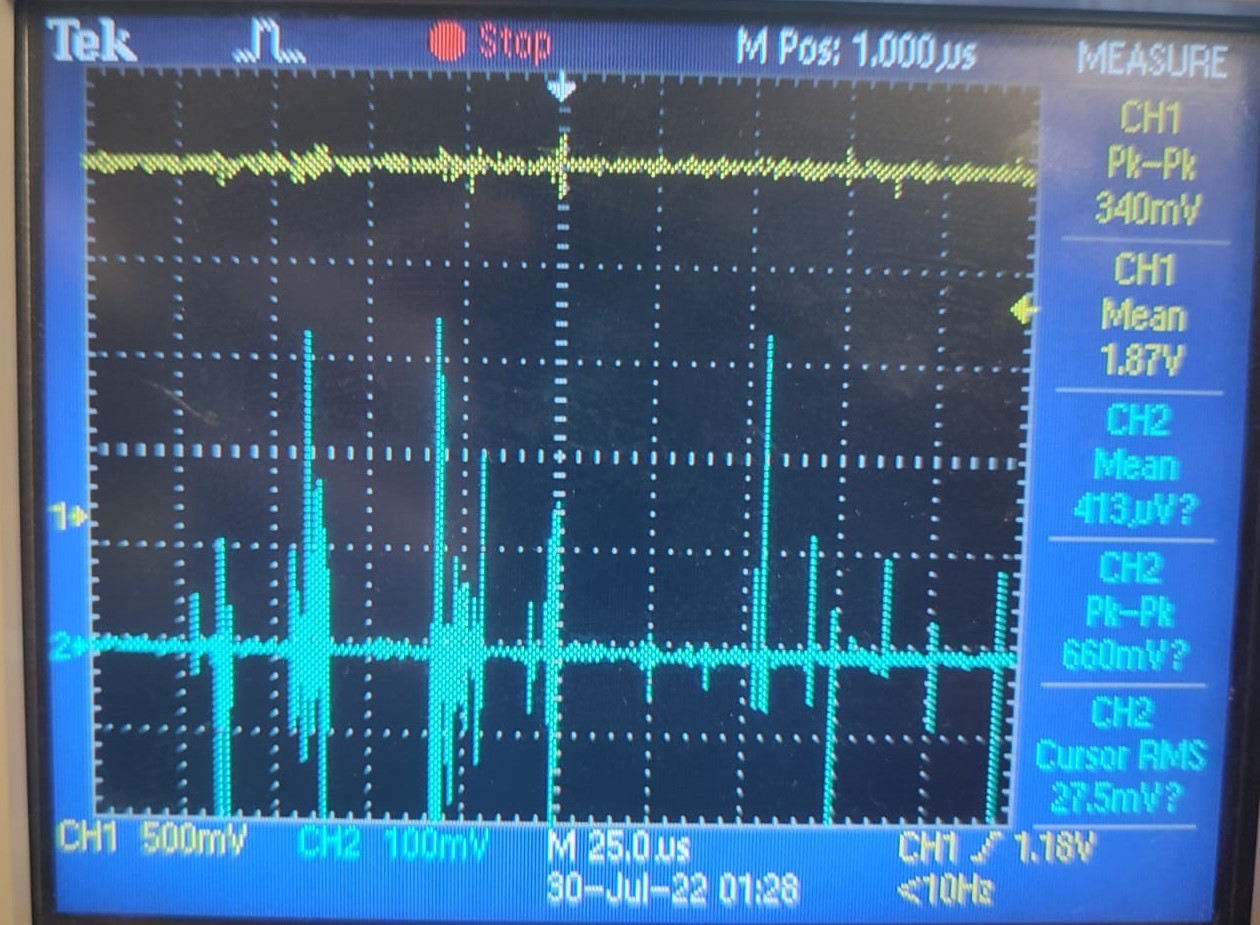
\includegraphics[width=\linewidth]{./Figures/CurSens_Prac_Slight.jpeg}
\caption{Circuit response to slight restriction on the motor.}
\label{subfig:cursen_prac_slight}	
\end{subfigure}
\vfill
\begin{subfigure}[]{0.3\textwidth}
\includegraphics[width=\linewidth]{./Figures/CurSens_Prac_Stall.jpeg}
\caption{Circuit response to motor stall.}
\label{subfig:cursen_prac_stall}	
\end{subfigure}
\hfill
\begin{subfigure}[]{0.3\textwidth}
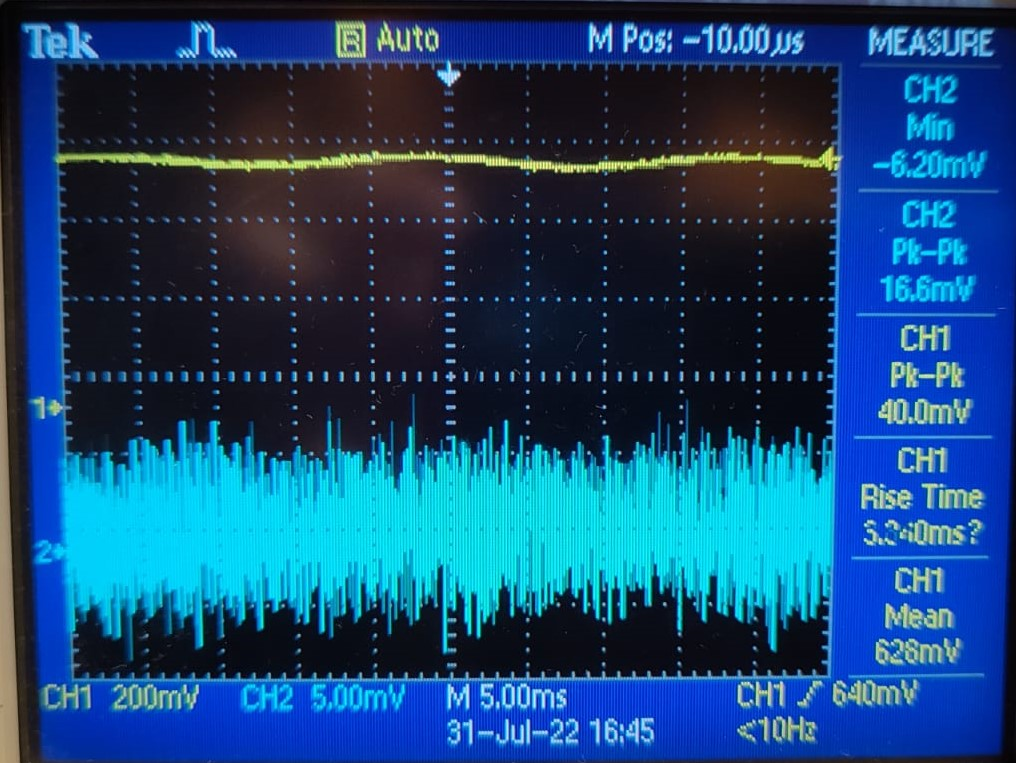
\includegraphics[width=\linewidth]{./Figures/CurSens_Prac_Noise.jpeg}
\caption{Circuit response to noise.}
\label{subfig:cursen_prac_noise}	
\end{subfigure}
\hfill
\begin{subfigure}[]{0.3\textwidth}
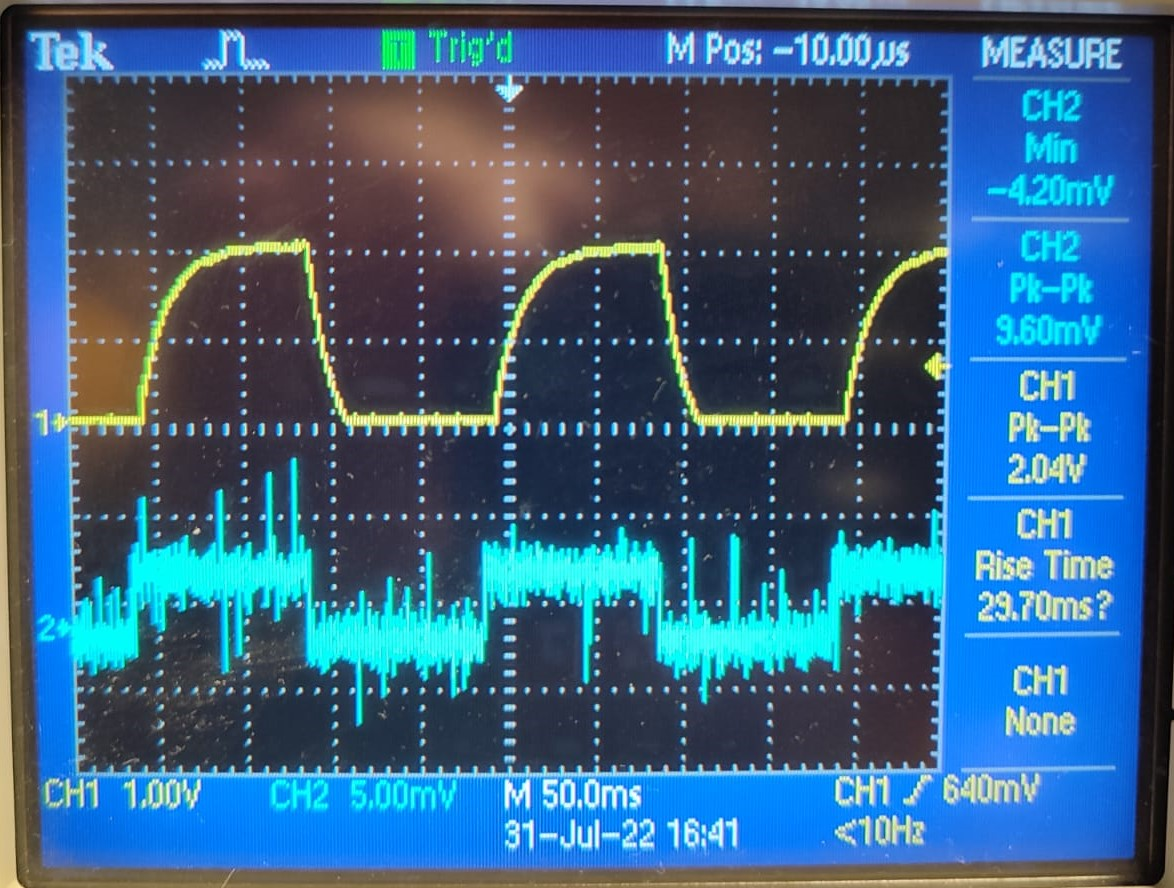
\includegraphics[width=\linewidth]{./Figures/CurSens_Prac_Step.jpeg}
\caption{Circuit response to step input.} 			
\label{subfig:cursen_prac_step}	
\end{subfigure}
\caption{Circuit response to different input conditions}
\label{fig:cursen_prac_resp}
\end{figure}

\clearpage
\section{Ultrasonic range sensor}
\subsection{Simulation}

Figure: \ref{fig:sonicsen_sim_step} shows the circuit response to a step input change from the maximum 10\% duty cycle to a 0.5\% duty cycle. As shown in the figure the circuit outputs > \SI{3}{\volt} for a maximum input and < \SI{0.3}{\volt} for the minimum input. The figure also demonstrates the circuits compliance to the noise and response time requirements with noise levels of \SI{58}{\milli\volt}pk-pk and a response time of \SI{386}{\milli\second}.

Figure: \ref{fig:sonicsen_sim_cur} shows that throughout circuit operation current draw is < \SI{170}{\micro\ampere}.

\begin{figure}[H]
\centering
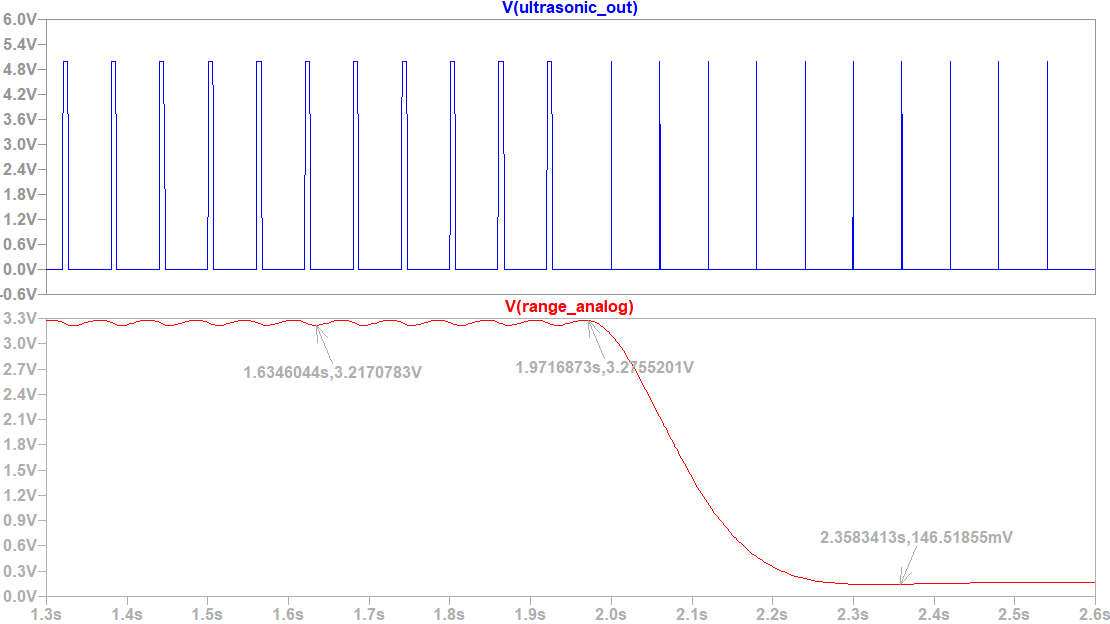
\includegraphics[width = 0.5\textwidth]{./Figures/SonicSens_RangeStep.png}
\caption{Circuit response to a full range step from 10\% to 0.5\% duty cycle}
\label{fig:sonicsen_sim_step}
\end{figure}

\begin{figure}[H]
\centering
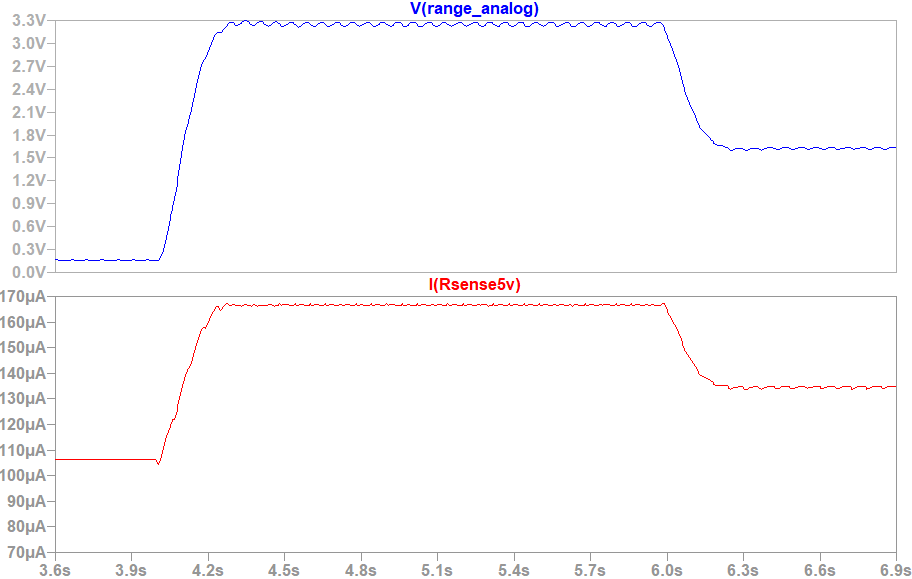
\includegraphics[width = 0.5\textwidth]{./Figures/SonicSens_CurDraw.png}
\caption{Current draw vs circuit output}
\label{fig:sonicsen_sim_cur}
\end{figure}

\clearpage
\subsection{Practical}

Figure: \ref{fig:sonicsen_sim_step} shows the output response to a step change from \SI{1}{\meter} to \SI{5}{\centi\meter} back to \SI{1}{\meter}. The figure also shows the compliance to the requirements with the \SI{1}{\meter} measurement having an output of \SI{3.24}{\volt} and an output of \SI{200}{\milli\volt} at \SI{5}{\centi\meter}. The figure also shows a compliance with the rise time of \SI{258}{\milli\second}.

Figure: \ref{subfig:sonicsen_prac_ripple} shows that the output ripple voltage is less than \SI{70}{\milli\volt}pk-pk at \SI{1}{\meter} when the ripple voltage will be at its worst.

Figure: \ref{subfig:sonicsen_prac_range} shows the circuit response to a gradual change in the input across the full range from close to far.

\begin{figure}[H]
\centering
\begin{subfigure}[]{0.45\textwidth}
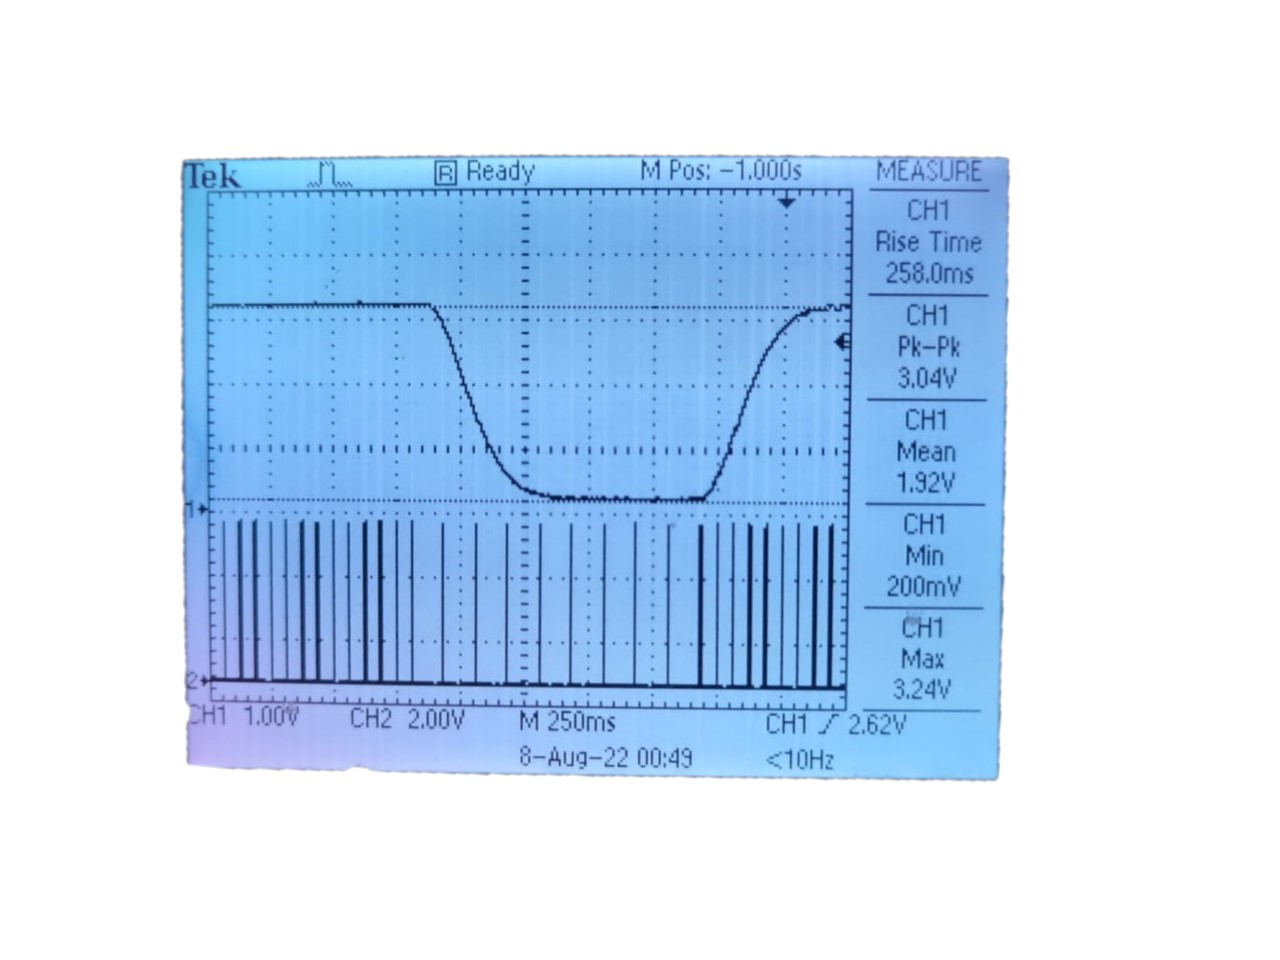
\includegraphics[width=\linewidth]{./Figures/SonicSens_Prac_Step.jpeg}
\caption{Circuit response a step input.}
\label{subfig:sonicsen_prac_step}	
\end{subfigure}
\hfill
\begin{subfigure}[]{0.45\textwidth}
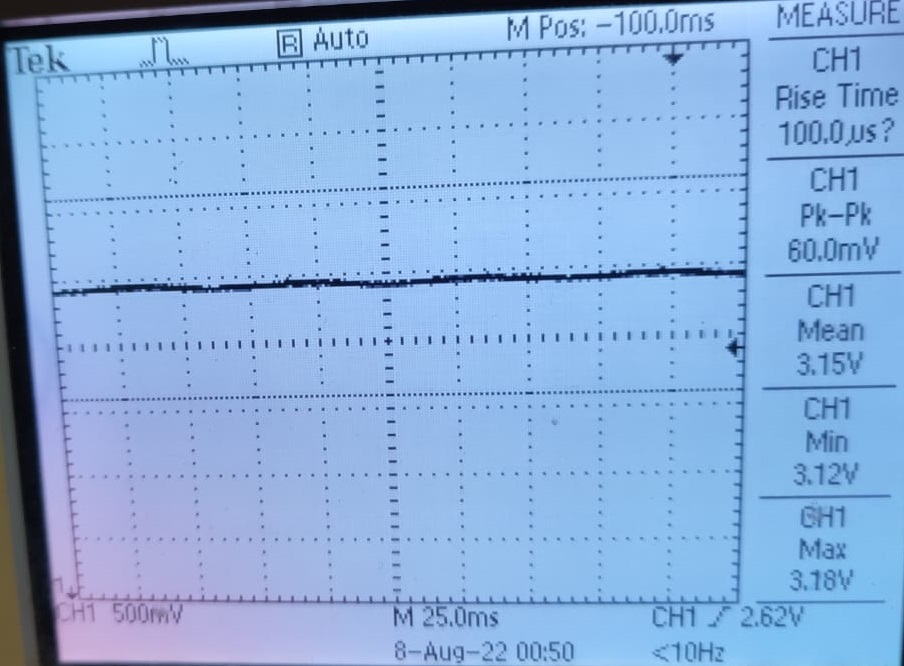
\includegraphics[width=\linewidth]{./Figures/SonicSens_Prac_Ripple.jpeg}
\caption{Circuit ripple voltage at 1m.} 			
\label{subfig:sonicsen_prac_ripple}	
\end{subfigure}
\vfill
\begin{subfigure}[]{0.45\textwidth}
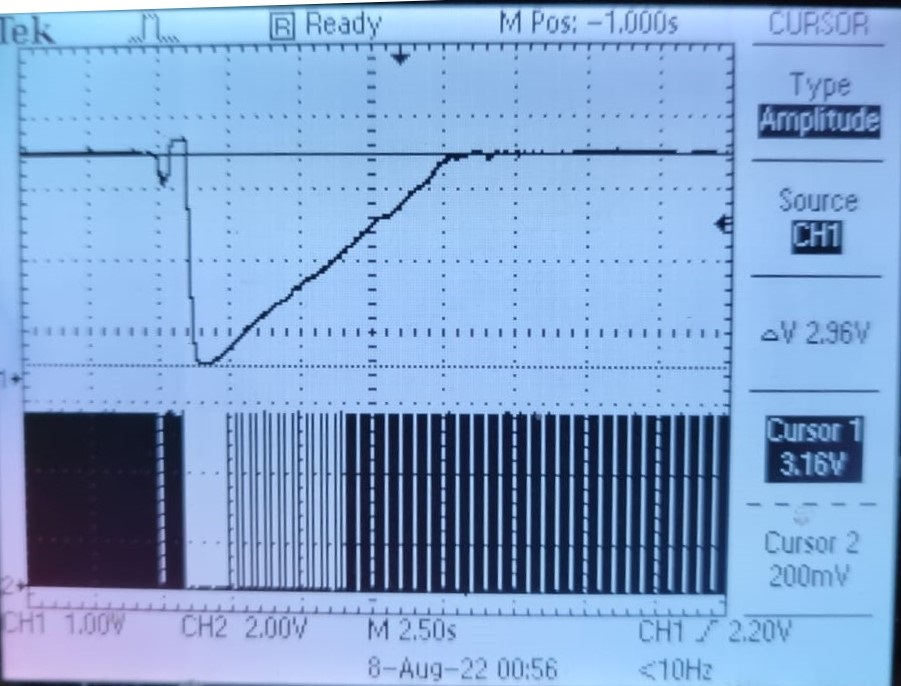
\includegraphics[width=\linewidth]{./Figures/SonicSens_Prac_Range.jpeg}
\caption{Circuit response to smooth change in range measurement.}
\label{subfig:sonicsen_prac_range}	
\end{subfigure}
\caption{Ultrasonic sensor filter circuit responses.}
\label{fig:sonicsen_prac}
\end{figure}


\clearpage
\section{Digital to analogue converter}
\subsection{Simulation}
Figure: \ref{fig:dac_sim_res} shows the simulation results and that the meet the specifications. 
\begin{figure}[H]
\centering
\begin{subfigure}{0.3\textwidth}
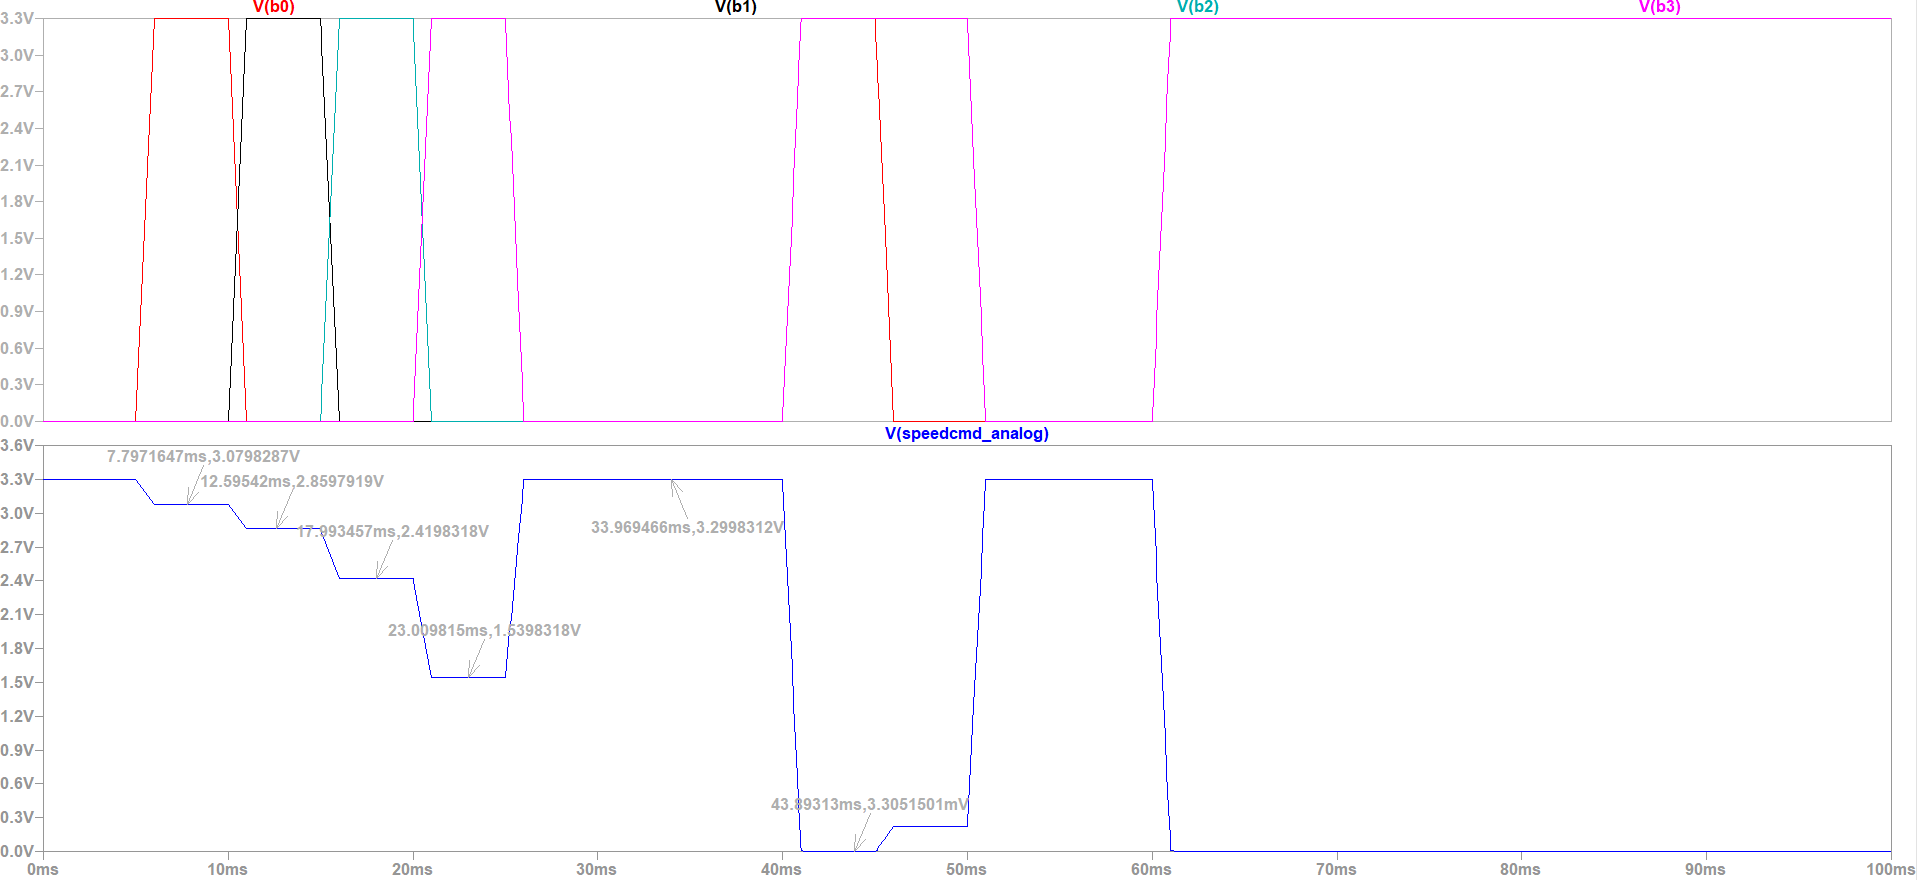
\includegraphics[width = \linewidth]{./Figures/DAC_Sim_Out.png}
\caption{Output vs input of DAC.}
\label{subfig:dac_sim_out}
\end{subfigure}
\hfill
\begin{subfigure}{0.3\textwidth}
\centering
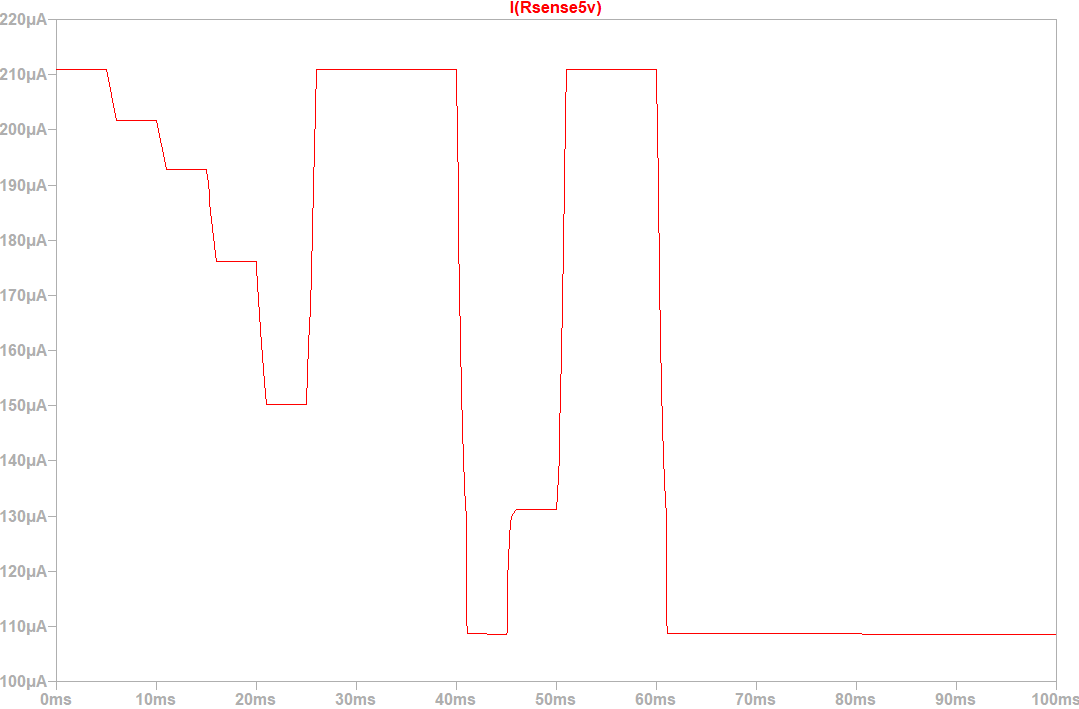
\includegraphics[width = \linewidth]{./Figures/DAC_Sim_Cur.png}
\caption{Current draw of the DAC circuit}
\label{subfig:dac_sim_cur}
\end{subfigure}
\caption{Simulation results of the DAC}
\label{fig:dac_sim_res}
\end{figure}

\subsection{Practical}
Figure: \ref{fig:dac_prac} shows the DAC response to different inputs and that the DAC meets all the given specifications.
\begin{figure}[H]
\centering
\begin{subfigure}[]{0.2\textwidth}
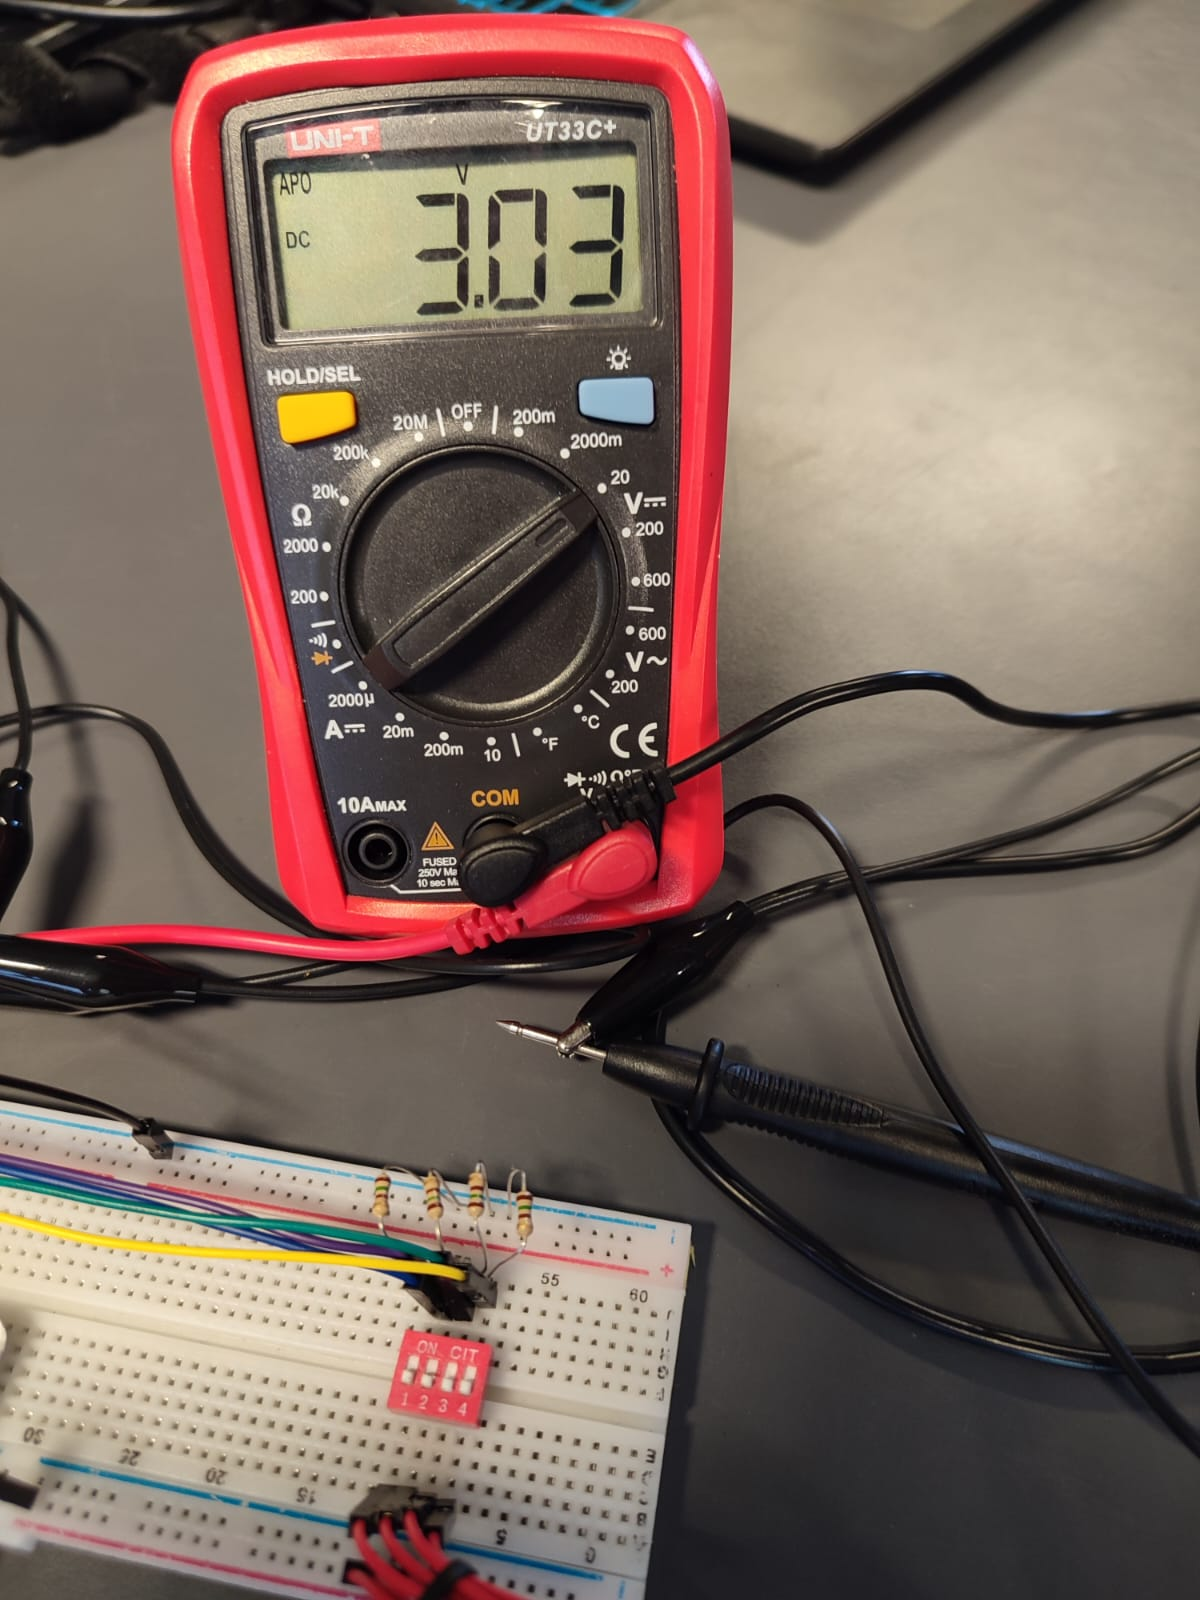
\includegraphics[width=\linewidth]{./Figures/DAC_Prac_0000.jpeg}
\caption{DAC output for 0000 input.}
\label{subfig:dac_prac_0000}	
\end{subfigure}
\hfill
\begin{subfigure}[]{0.2\textwidth}
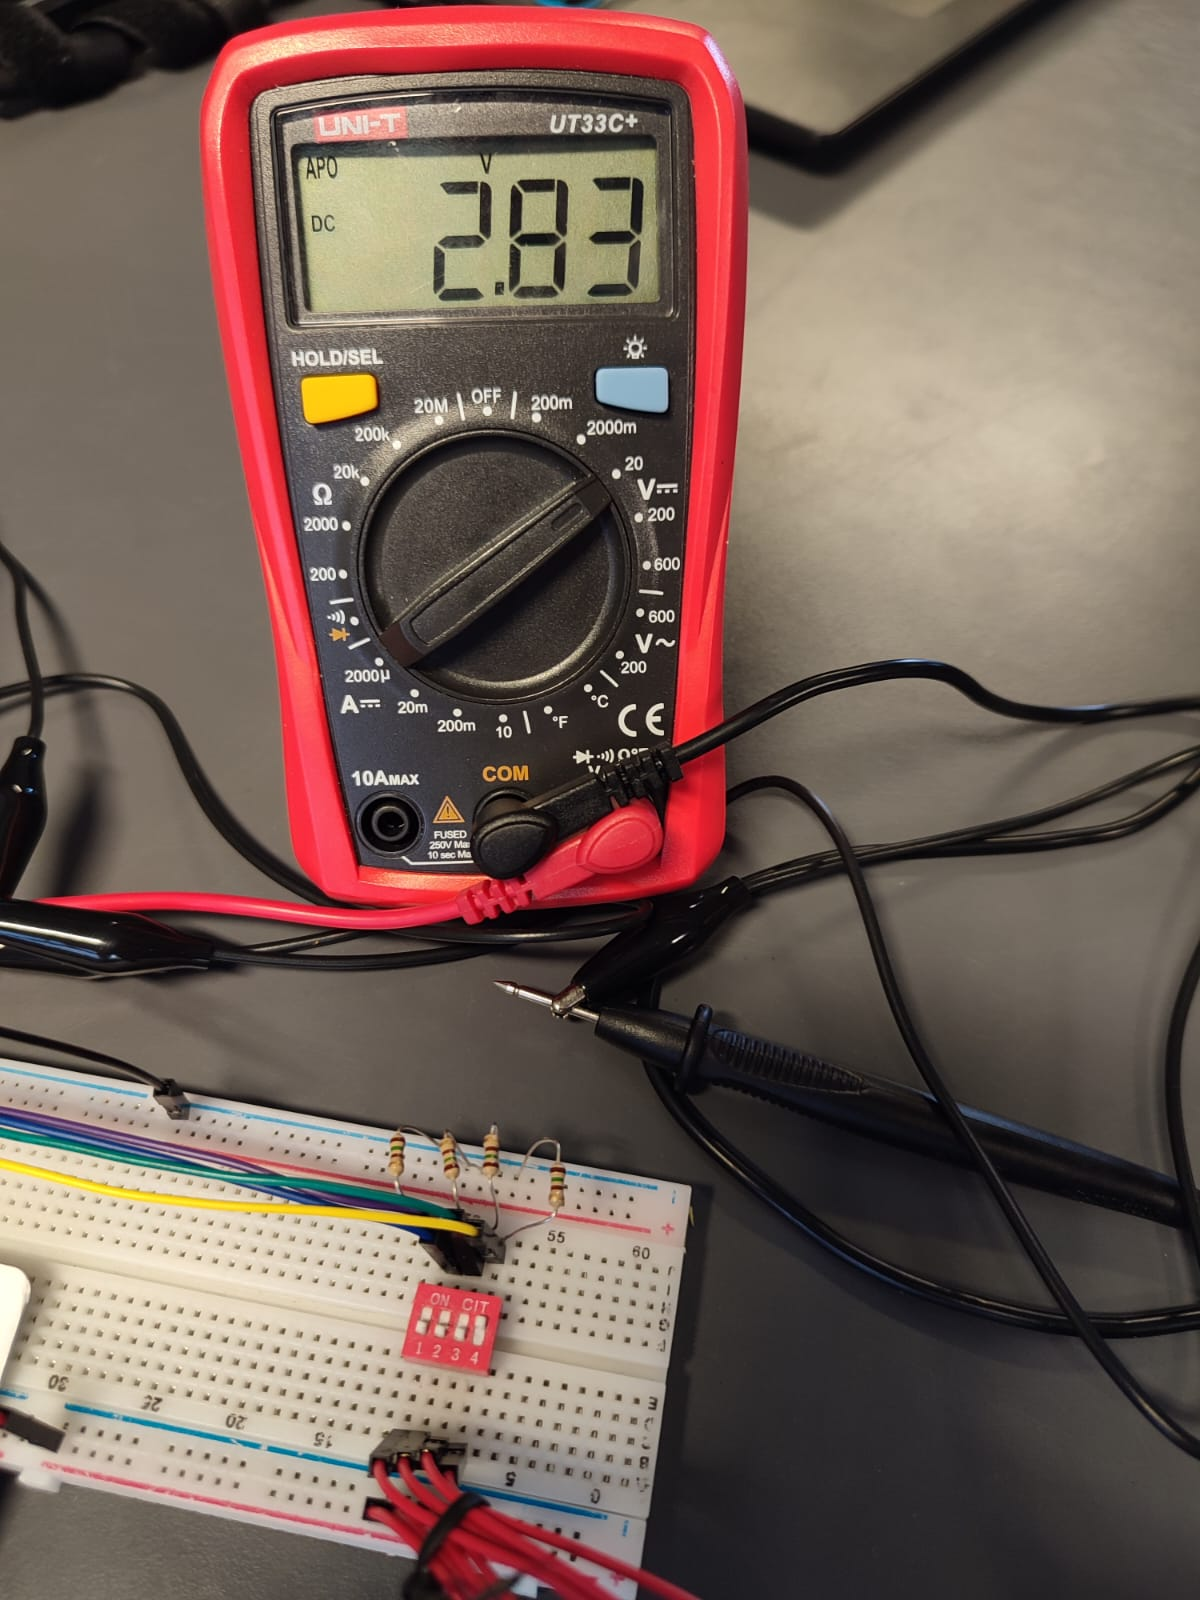
\includegraphics[width=\linewidth]{./Figures/DAC_Prac_0001.jpeg}
\caption{DAC output for 0001 input.} 			
\label{subfig:dac_prac_0001}	
\end{subfigure}
\hfill
\begin{subfigure}[]{0.2\textwidth}
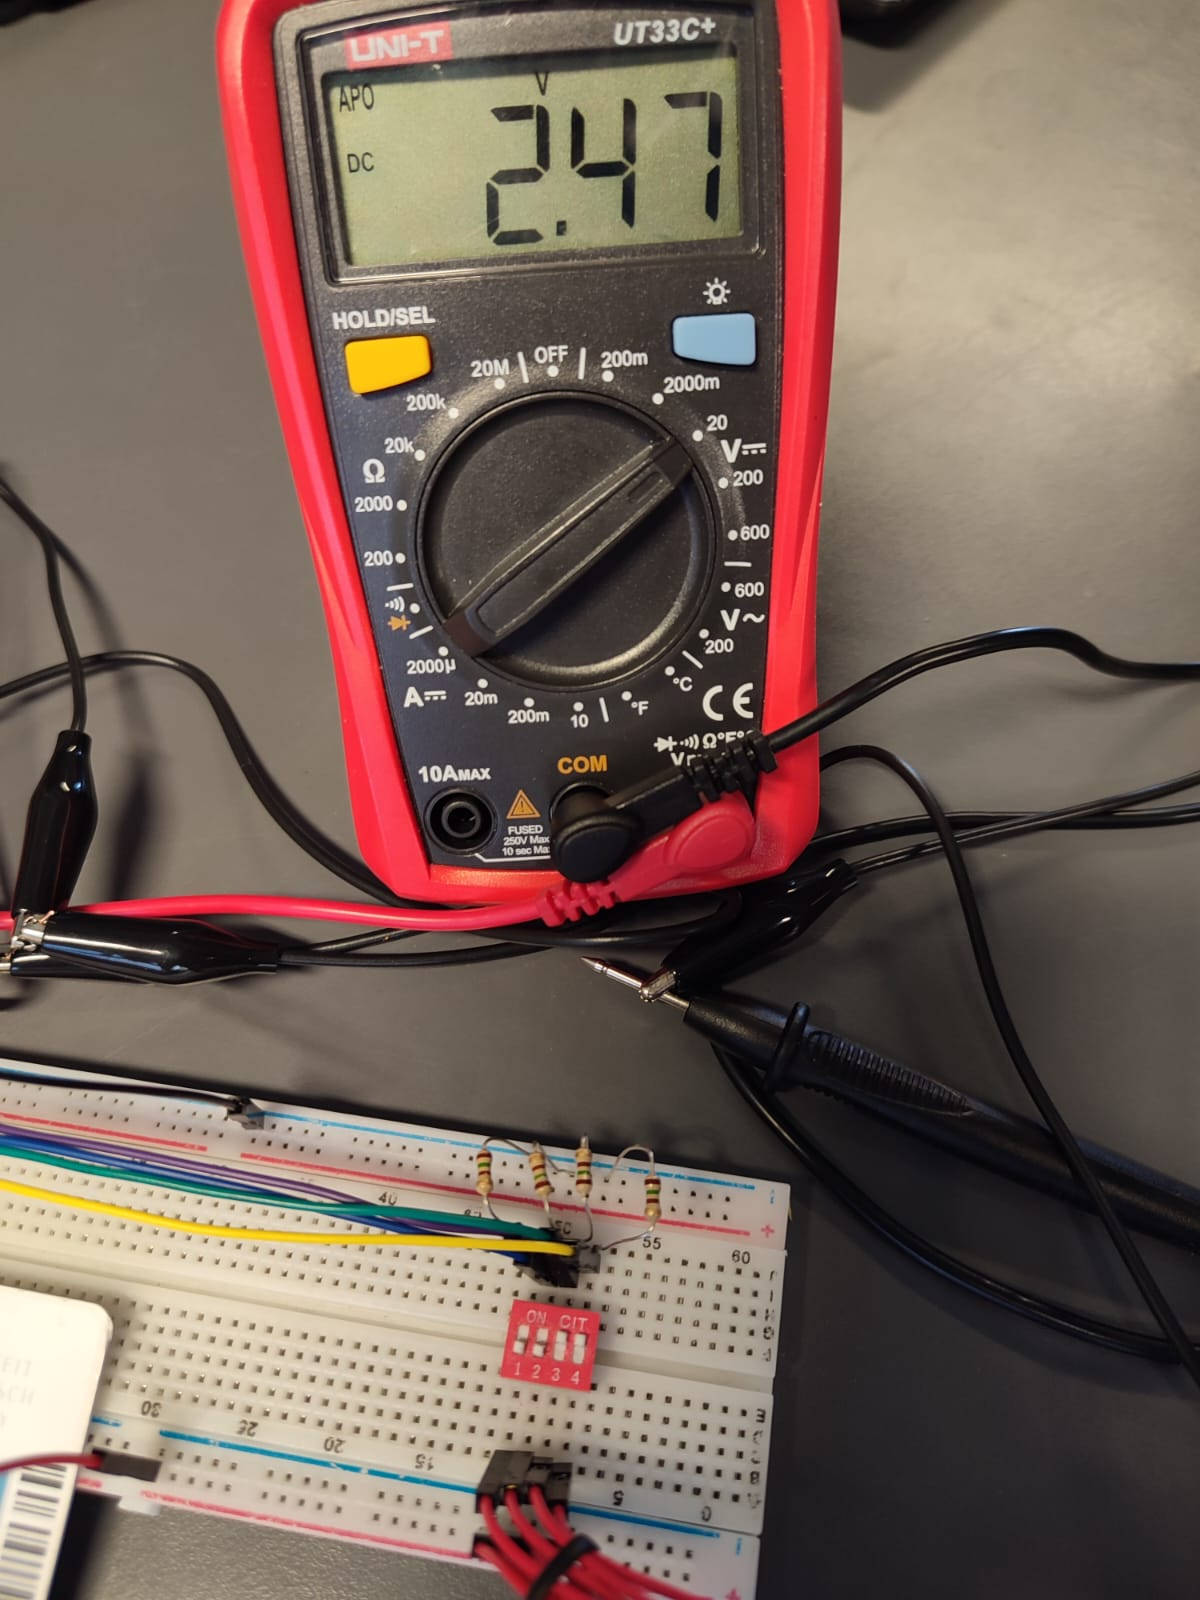
\includegraphics[width=\linewidth]{./Figures/DAC_Prac_0011.jpeg}
\caption{DAC output for 0011 input.} 			
\label{subfig:dac_prac_0011}	
\end{subfigure}
\vfill
\begin{subfigure}[]{0.2\textwidth}
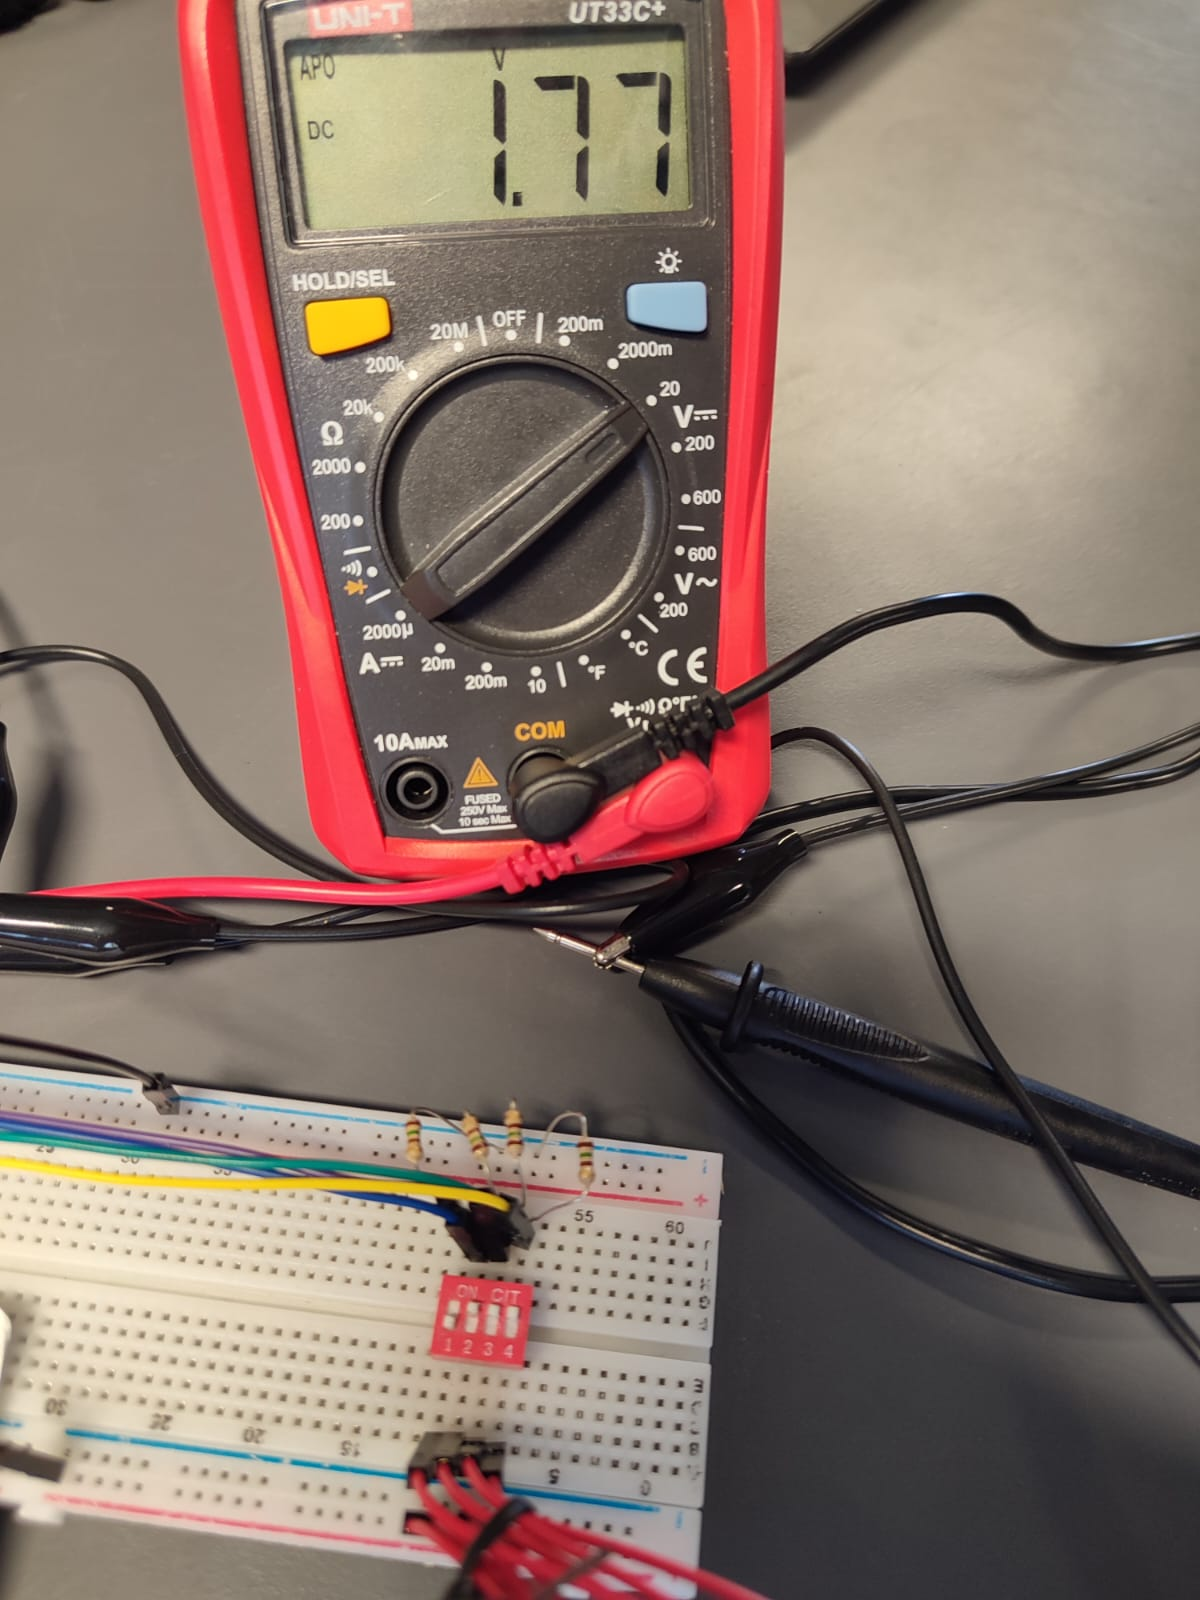
\includegraphics[width=\linewidth]{./Figures/DAC_Prac_0111.jpeg}
\caption{DAC output for 0111 input.}
\label{subfig:dac_prac_0111}	
\end{subfigure}
\hfill
\begin{subfigure}[]{0.2\textwidth}
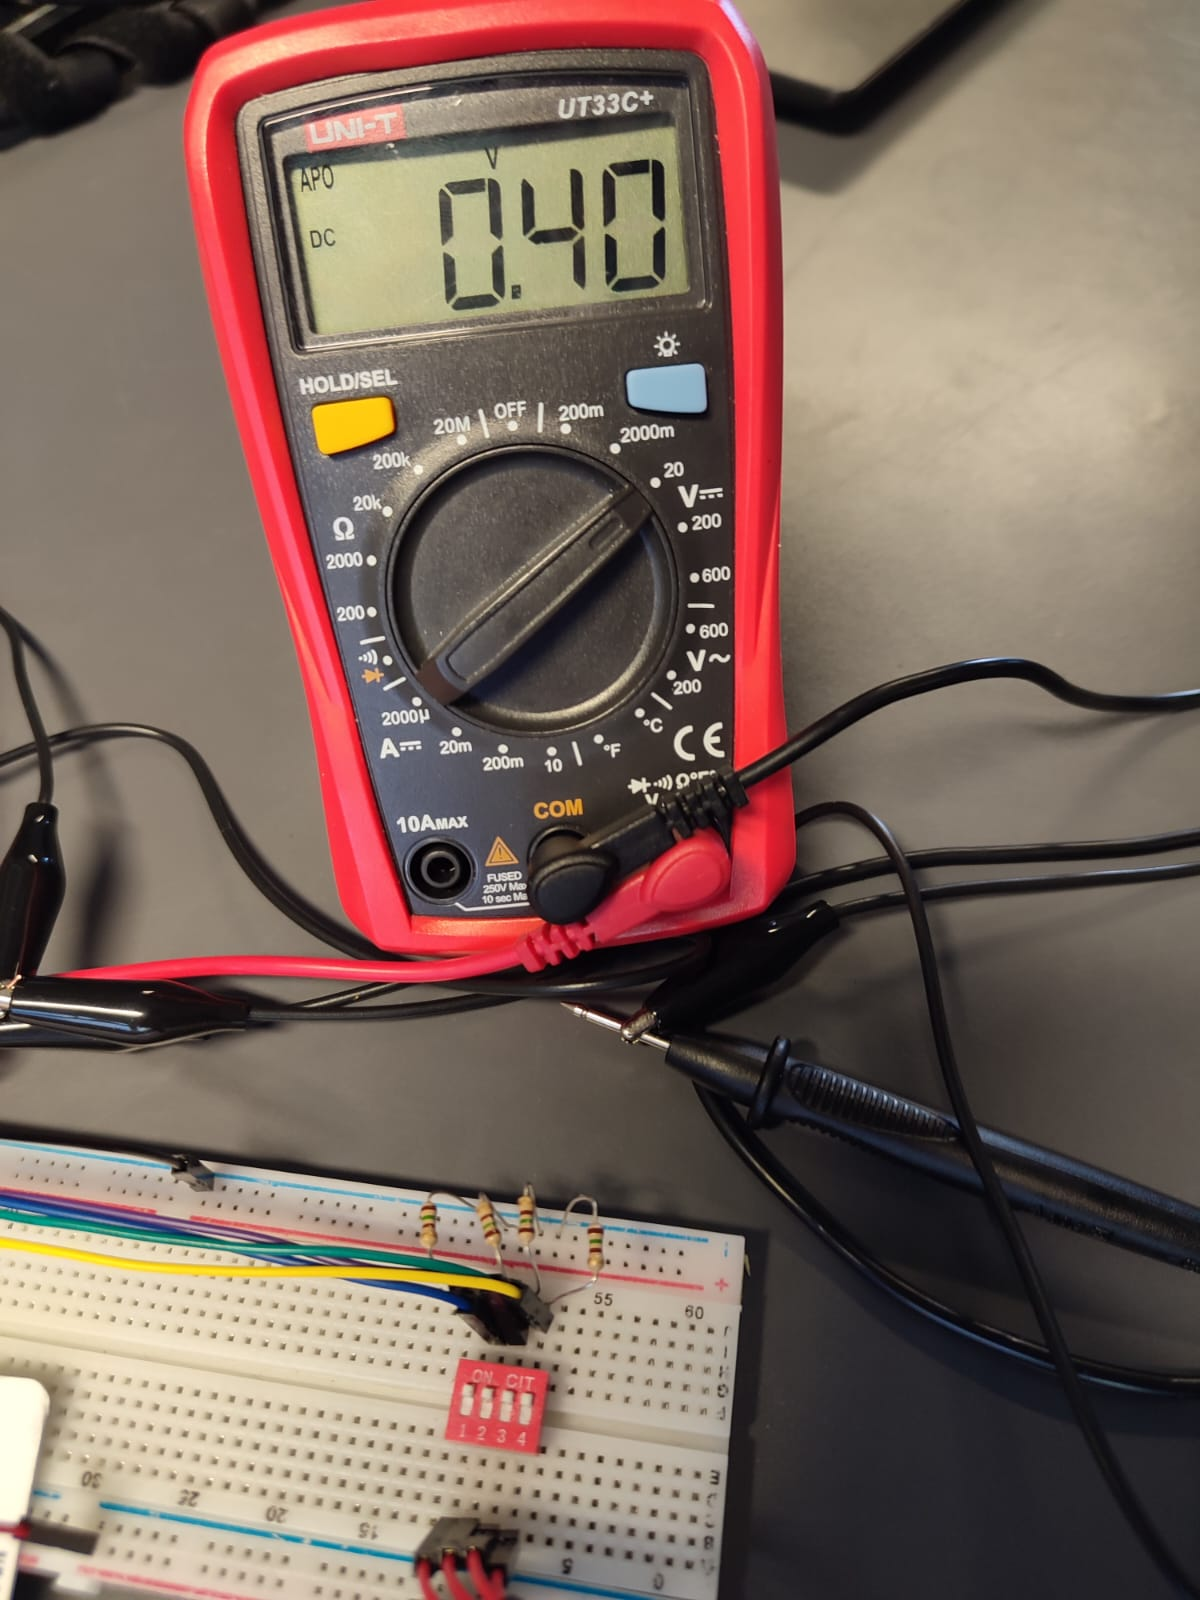
\includegraphics[width=\linewidth]{./Figures/DAC_Prac_1111.jpeg}
\caption{DAC output for 1111 input.}
\label{subfig:dac_prac_1111}
\end{subfigure}
\hfill
\begin{subfigure}[]{0.2\textwidth}
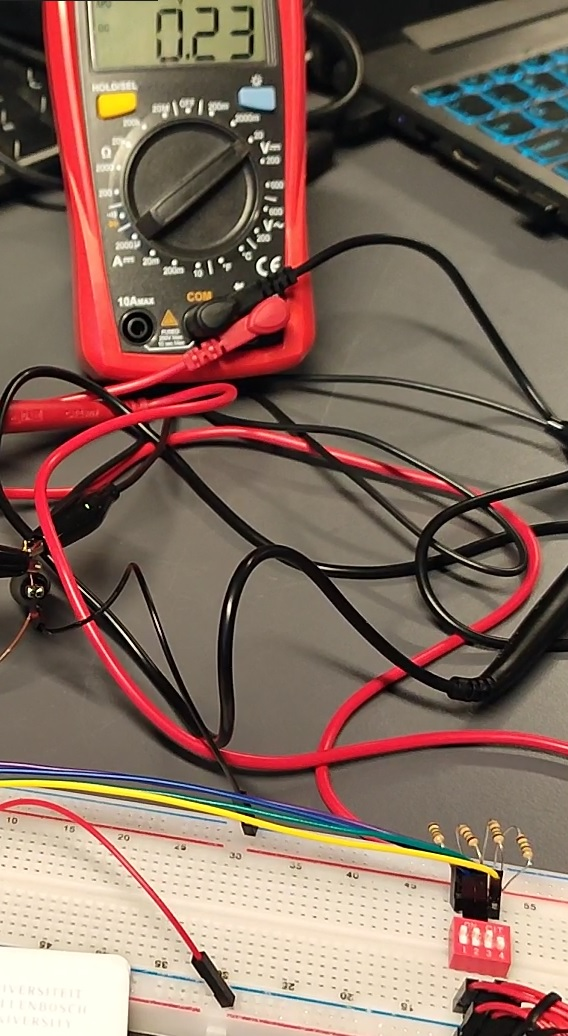
\includegraphics[width=\linewidth]{./Figures/DAC_Prac_1110.jpeg}
\caption{DAC output for 1110 input.} 			
\label{subfig:dac_prac_1110}	
\end{subfigure}
\caption{DAC output for different inputs.}
\label{fig:dac_prac}
\end{figure}

\clearpage
\section{Motor Control}
\subsection{Simulation}
\begin{figure}[H]
\centering
\begin{subfigure}[]{0.4\textwidth}
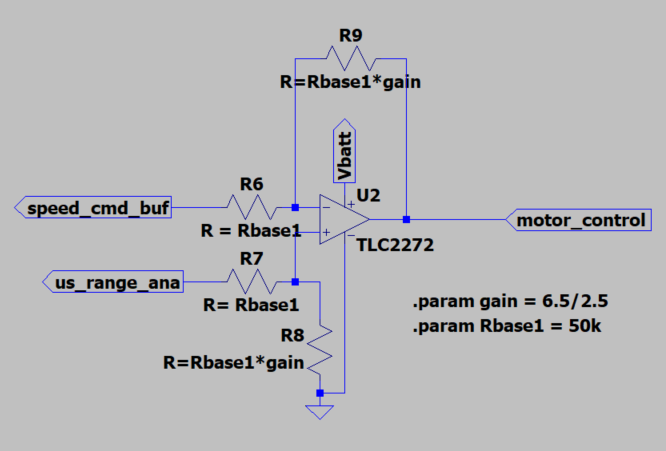
\includegraphics[width=\linewidth]{./Figures/Mtr_Ctrl_Sub_Cir.png}
\caption{Circuit diagram for the subtracting circuit.}
\label{subfig:mtrctrl_sub_cir}	
\end{subfigure}
\hfill
\begin{subfigure}[]{0.4\textwidth}
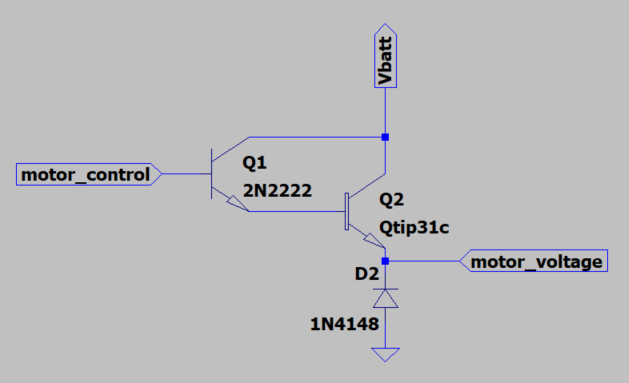
\includegraphics[width=\linewidth]{./Figures/Mtr_Ctrl_Darling_Cir.png}
\caption{Circuit diagram for the Darlington pair.} 			
\label{subfig:mtrctrl_darling_cir}	
\end{subfigure}
\caption{Circuits used for motor control.}
\label{fig:mtrctrl_cir}
\end{figure}

\begin{figure}[H]
\centering
\begin{subfigure}[]{0.4\textwidth}
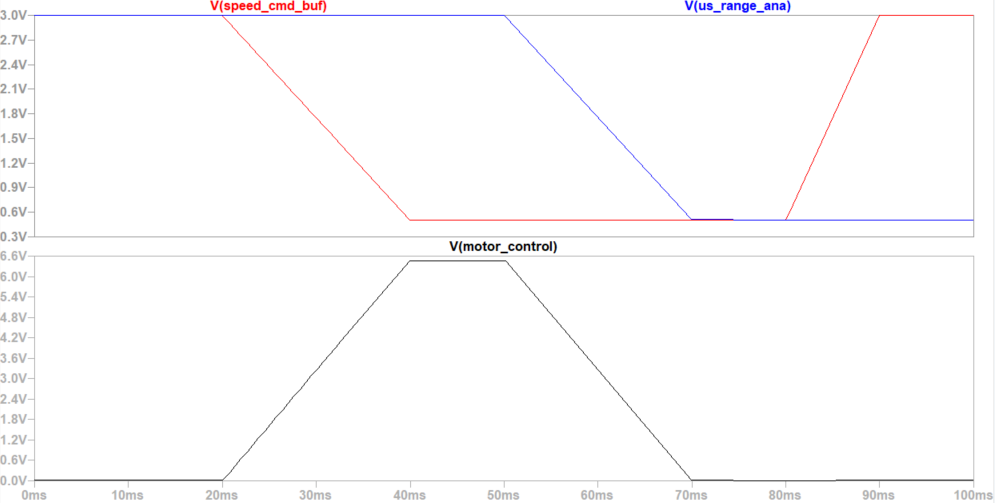
\includegraphics[width=\linewidth]{./Figures/Mtr_Ctrl_Sub_Out.png}
\caption{Output vs input for the subtracting op amp.}
\label{subfig:mtrctrl_sub_out}	
\end{subfigure}
\hfill
\begin{subfigure}[]{0.4\textwidth}
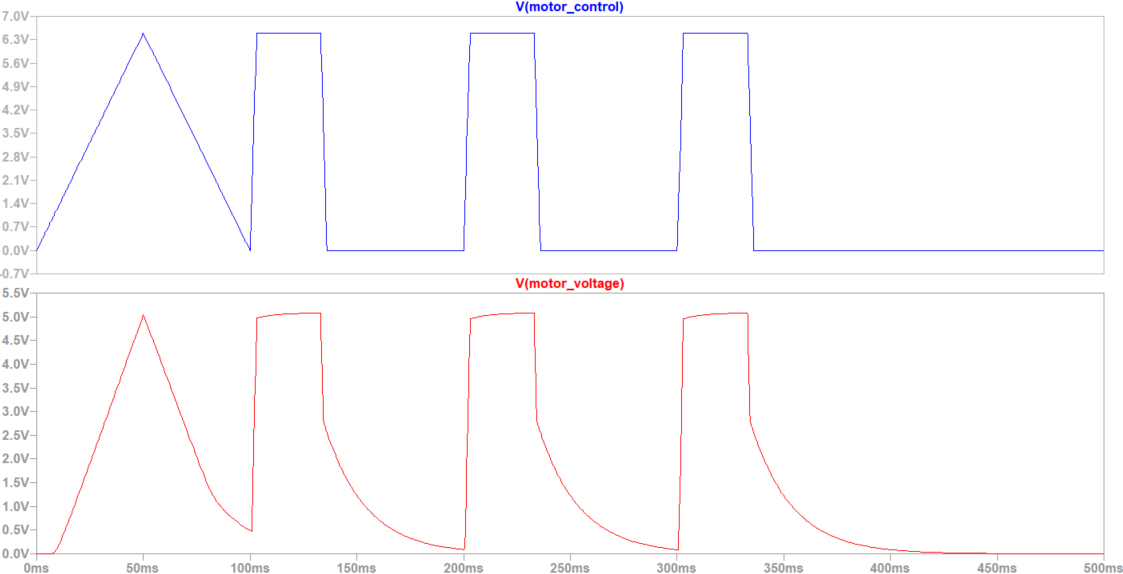
\includegraphics[width=\linewidth]{./Figures/Mtr_Ctrl_Darling_Out.png}
\caption{Output for the Darlington pair.} 			
\label{subfig:mtrctrl_darling_out}	
\end{subfigure}
\caption{Simulated circuit responses.}
\label{fig:mtrctrl_out}
\end{figure}


\clearpage
\subsection{Practical}
\begin{figure}[H]
\centering
\begin{subfigure}[]{0.4\textwidth}
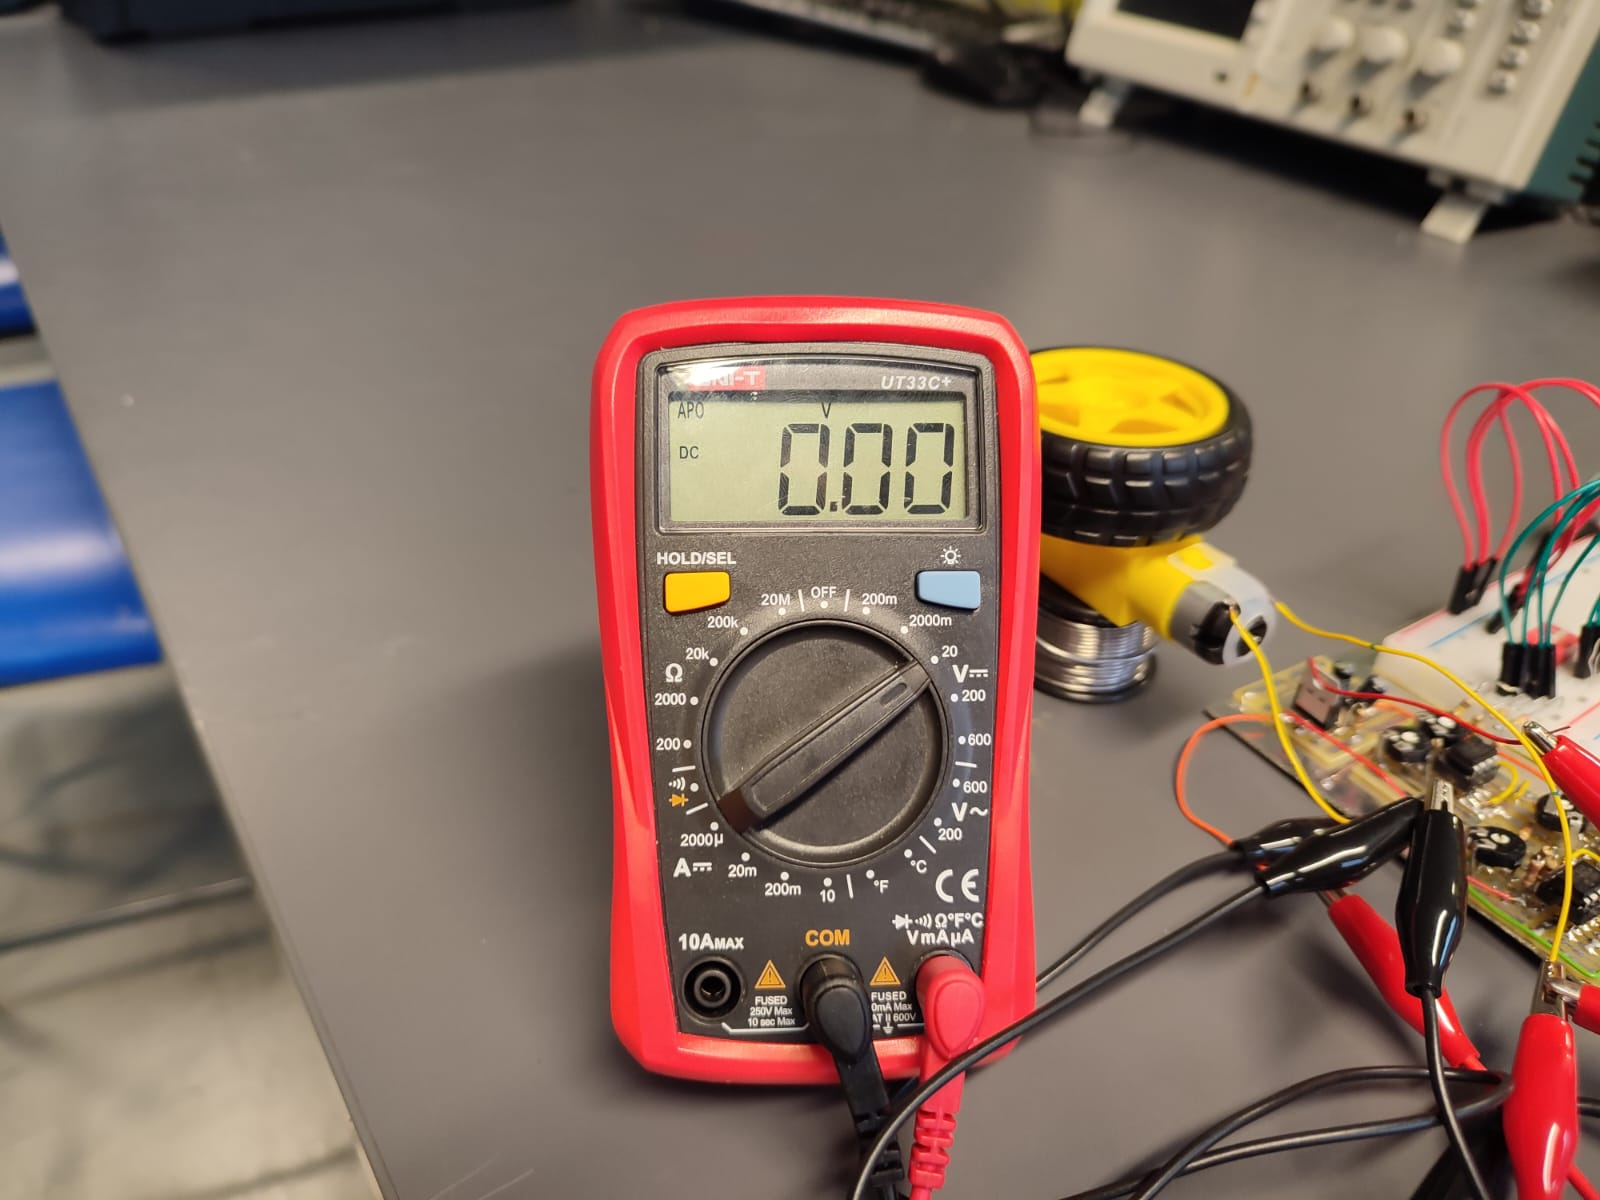
\includegraphics[width=\linewidth]{./Figures/Mtr_Ctrl_Slow_Far.jpeg}
\caption{Slow speed command and far object.}
\label{subfig:mtrctrl_prac_sf}	
\end{subfigure}
\hfill
\begin{subfigure}[]{0.4\textwidth}
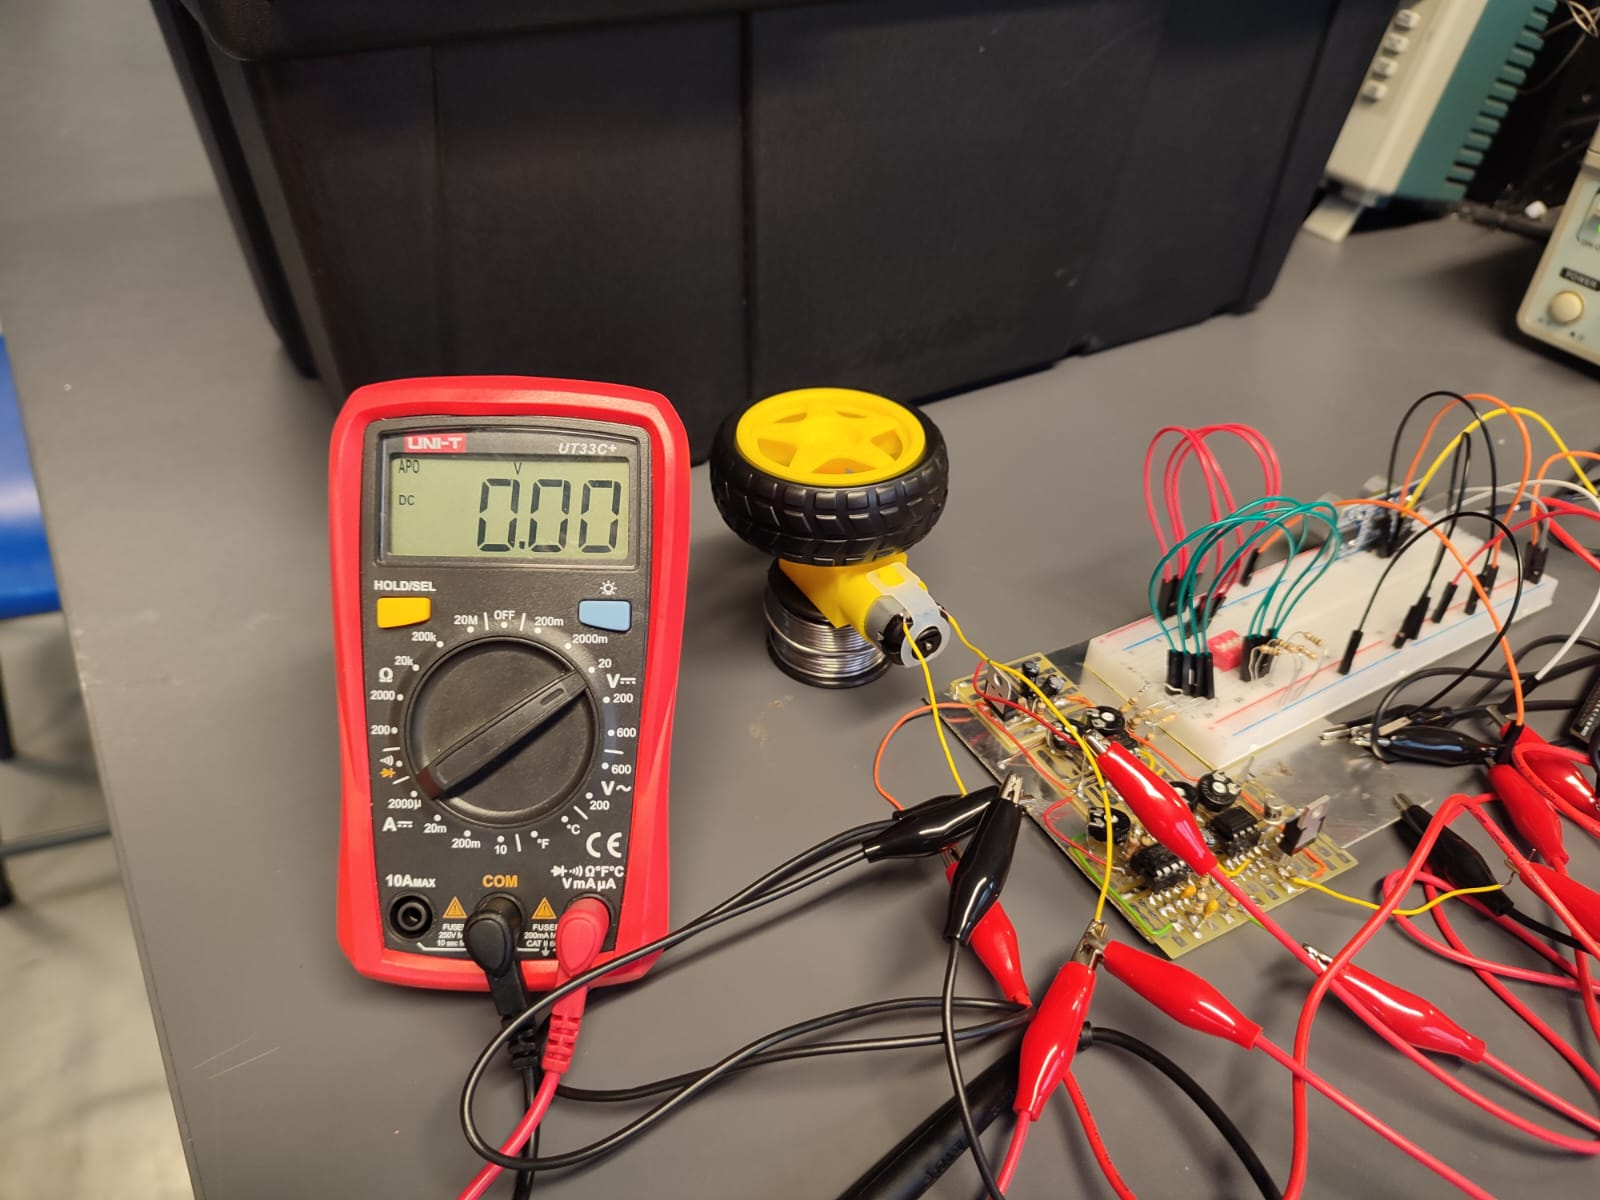
\includegraphics[width=\linewidth]{./Figures/Mtr_Ctrl_Slow_Close.jpeg}
\caption{Slow speed command and close object.} 			
\label{subfig:mtrctrl_prac_sc}	
\end{subfigure}
\begin{subfigure}[]{0.4\textwidth}
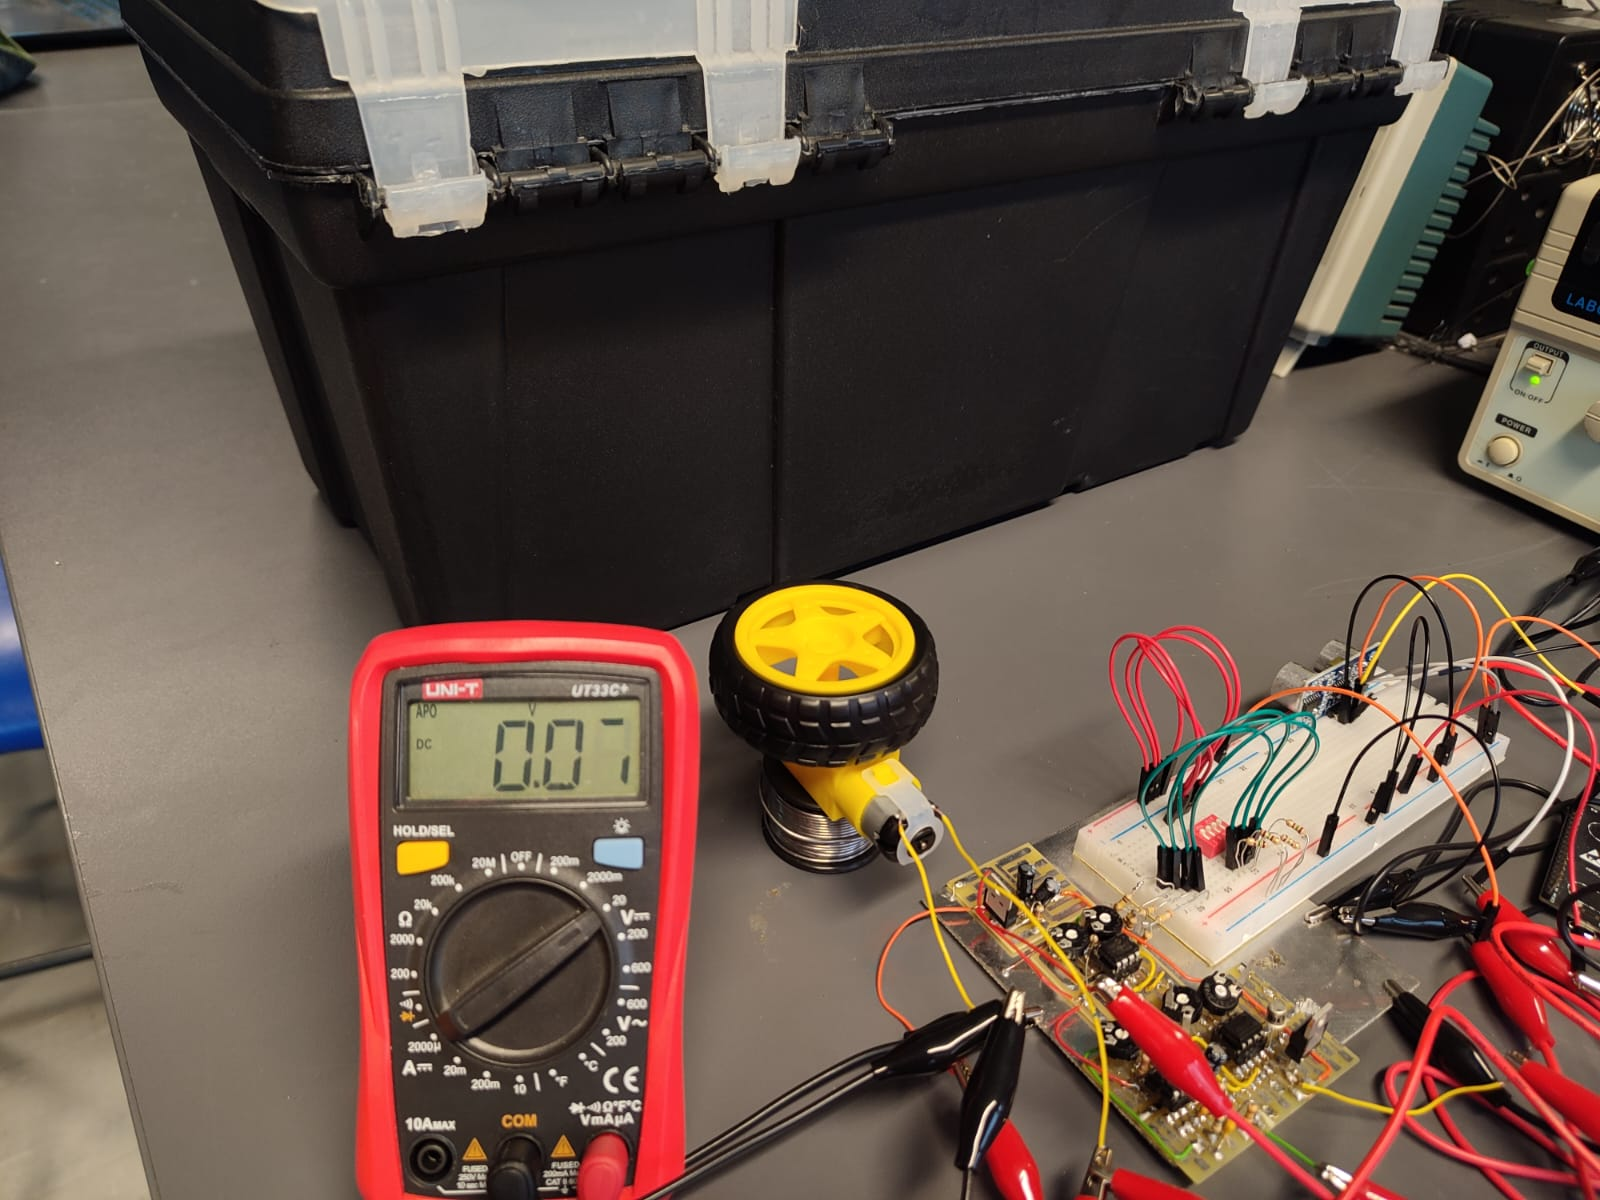
\includegraphics[width=\linewidth]{./Figures/Mtr_Ctrl_Fast_Close.jpeg}
\caption{Fast speed command and close object.}
\label{subfig:mtrctrl_prac_fc}	
\end{subfigure}
\hfill
\begin{subfigure}[]{0.4\textwidth}
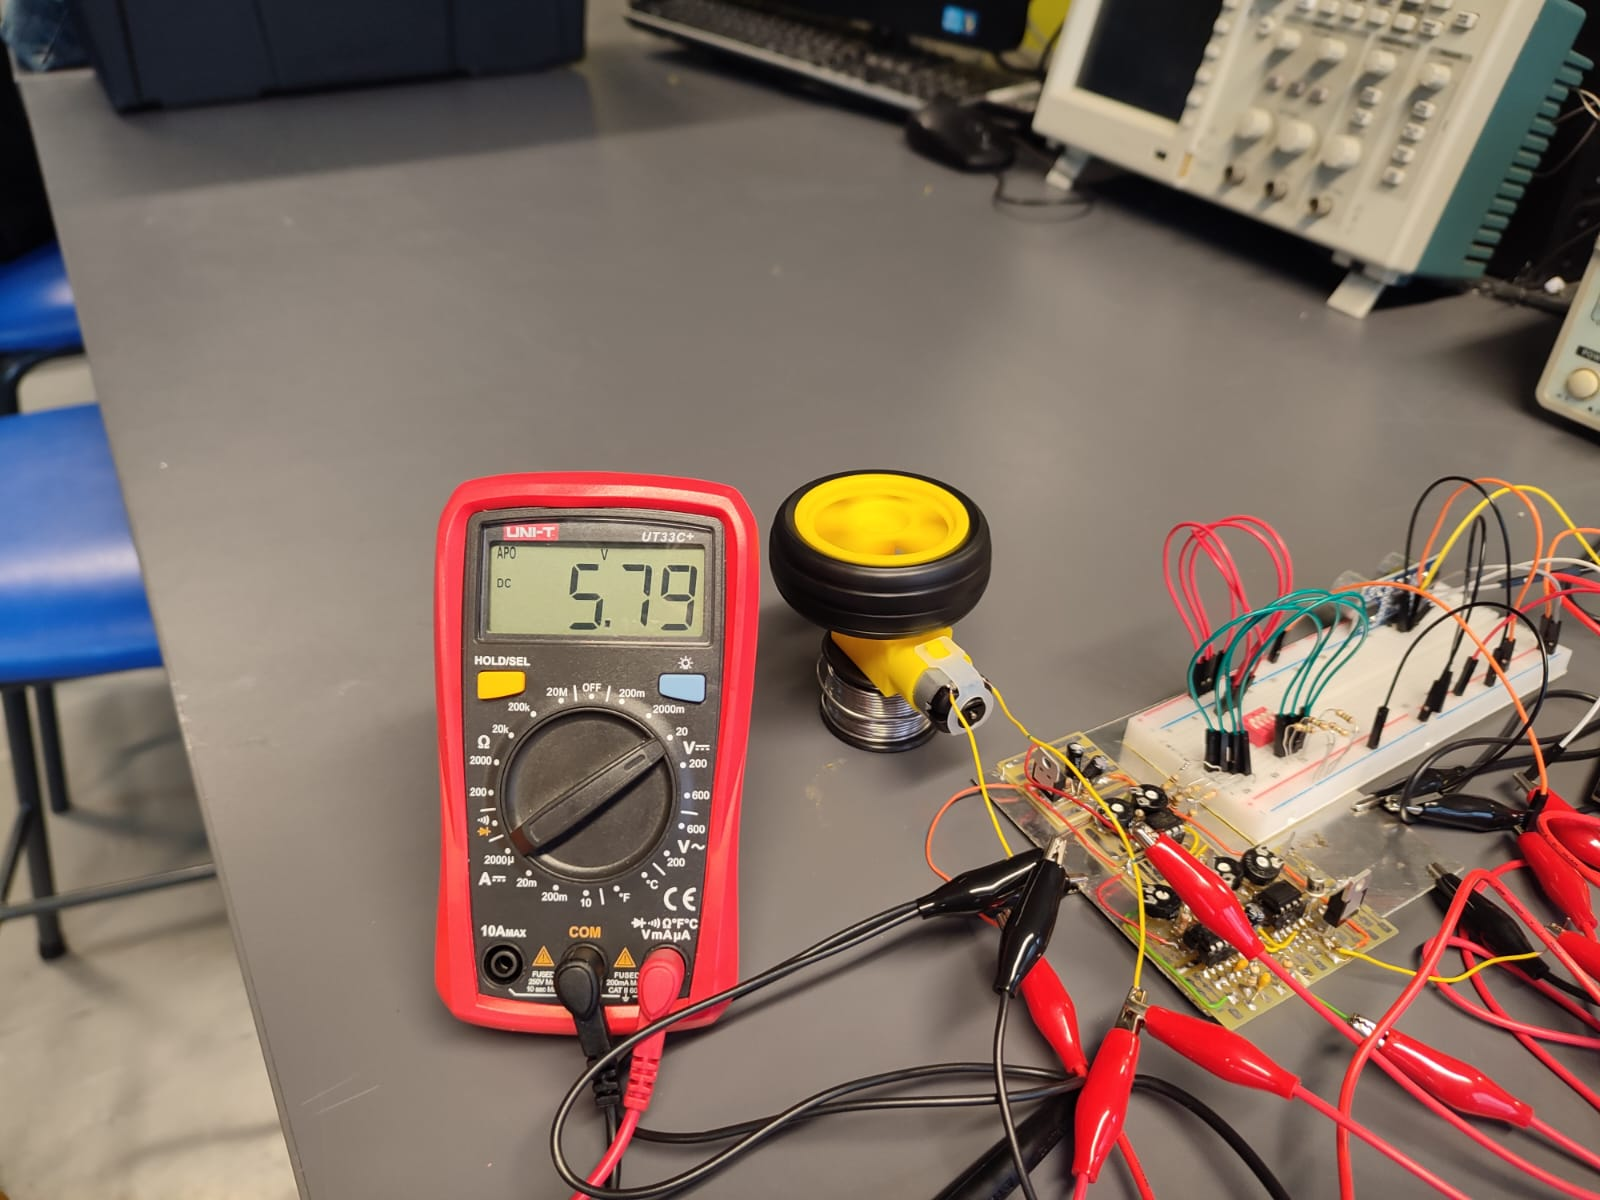
\includegraphics[width=\linewidth]{./Figures/Mtr_Ctrl_Fast_Far.jpeg}
\caption{Fast speed command and far object.} 			
\label{subfig:mtrctrl_prac_ff}	
\end{subfigure}
\caption{Motor voltage for different input conditions.}
\label{fig:mtrctrl_prac}
\end{figure}


\clearpage
\section{Voltage Regulation}
\begin{figure}[H]
\centering
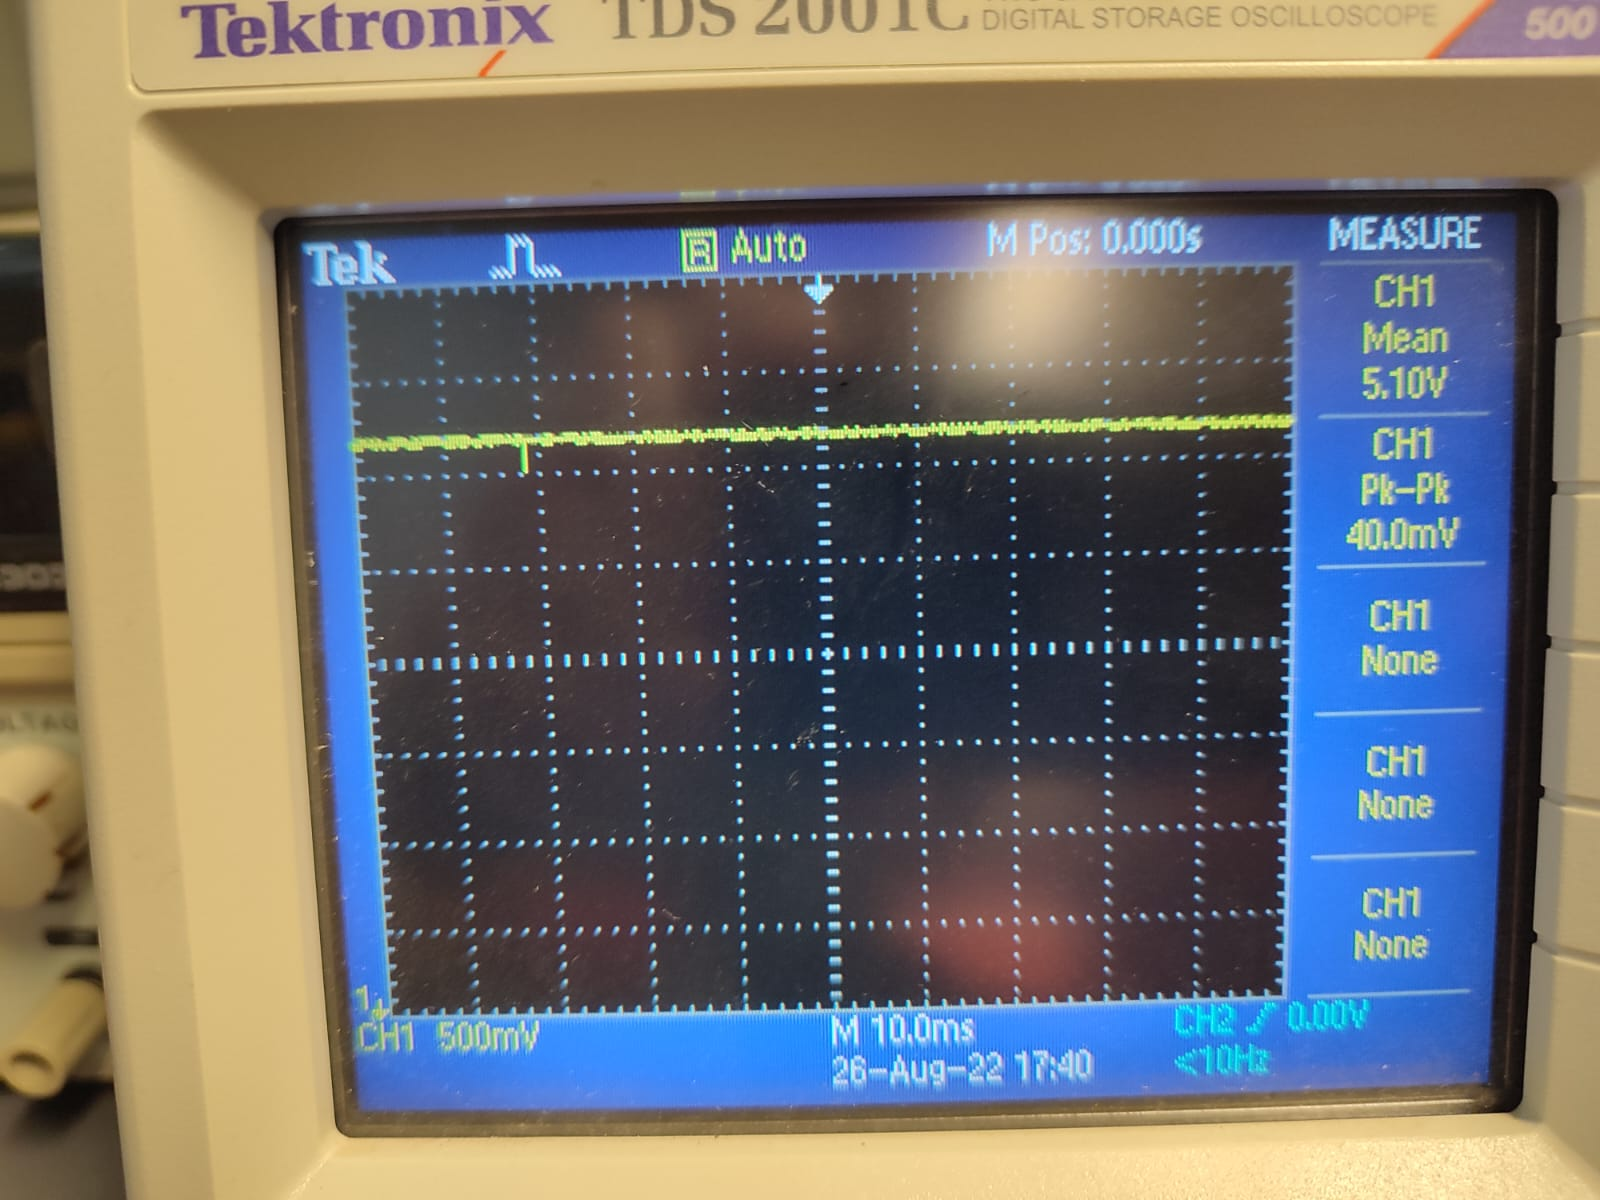
\includegraphics[width = 0.9\textwidth]{./Figures/Volt_Reg_Noise.jpeg}
\caption{Voltage regulator output}
\label{fig:volt_reg_noise}
\end{figure}

\clearpage
\section{Left side wheel control}
\subsection{Simulation results}
\subsubsection{Current Sensor}
\begin{figure}[H]
\centering
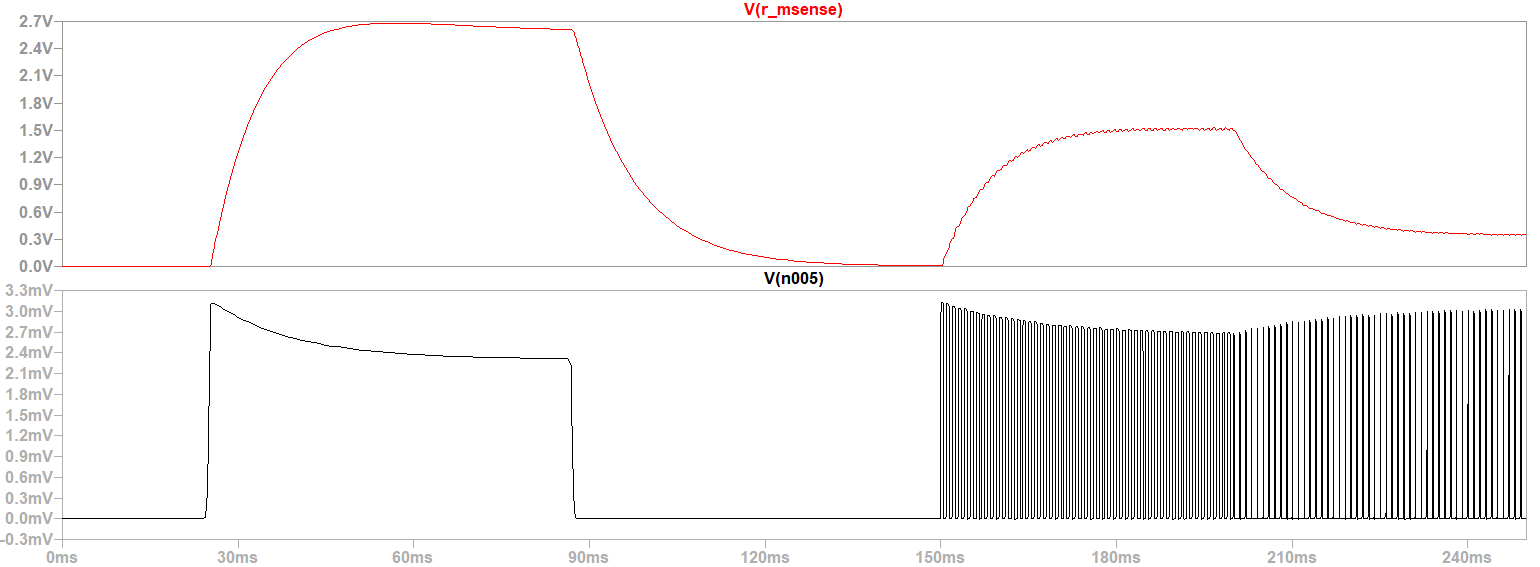
\includegraphics[width = 0.5\textwidth]{./Figures/CurSens_Left_Sim.png}
\caption{Current sensor output and current sensor resistor voltage}
\label{fig:CurSens_Left_Sim}
\end{figure}
\subsubsection{PWM control}
\begin{figure}[H]
\centering
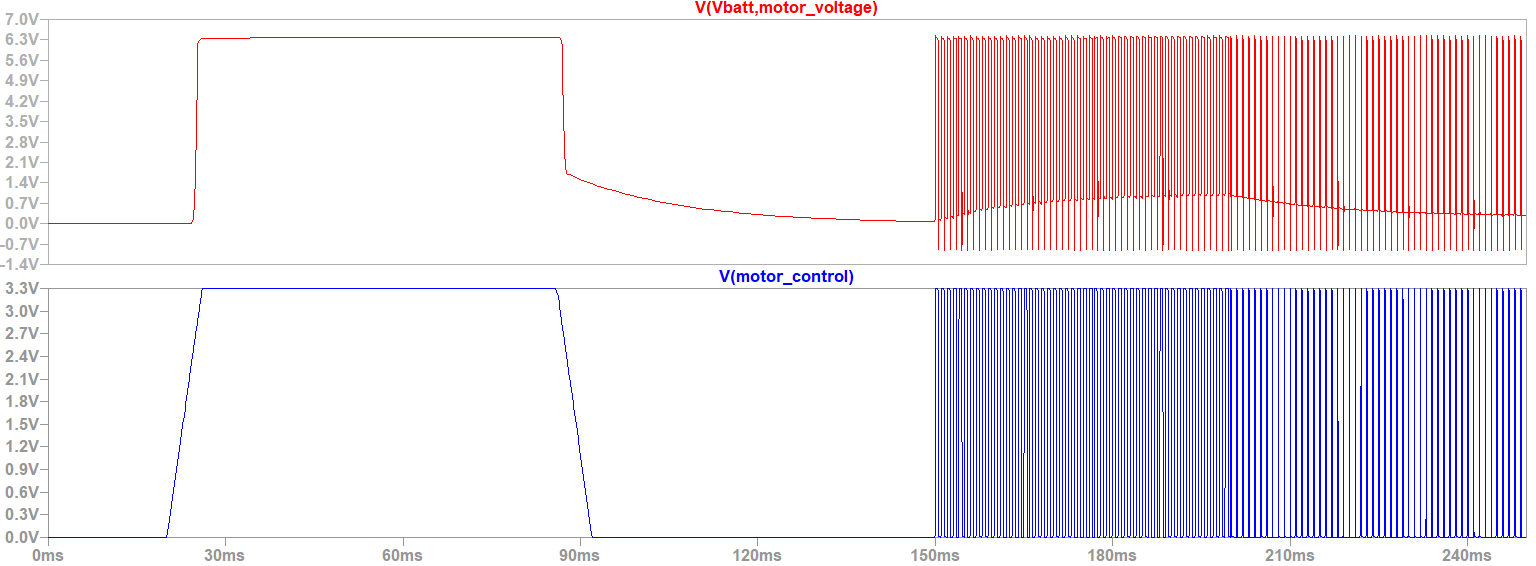
\includegraphics[width = 0.5\textwidth]{./Figures/PWM_Ctrl_Sim.png}
\caption{Motor voltage and Motor control signal}
\label{fig:PWM_ctrl_sim}
\end{figure}
\clearpage
\subsection{Practical results}
\subsubsection{Current Sensor}
\subsubsection{PWM control}

\clearpage
\section{Photo's of Circuits}
\begin{figure}[H]
\centering
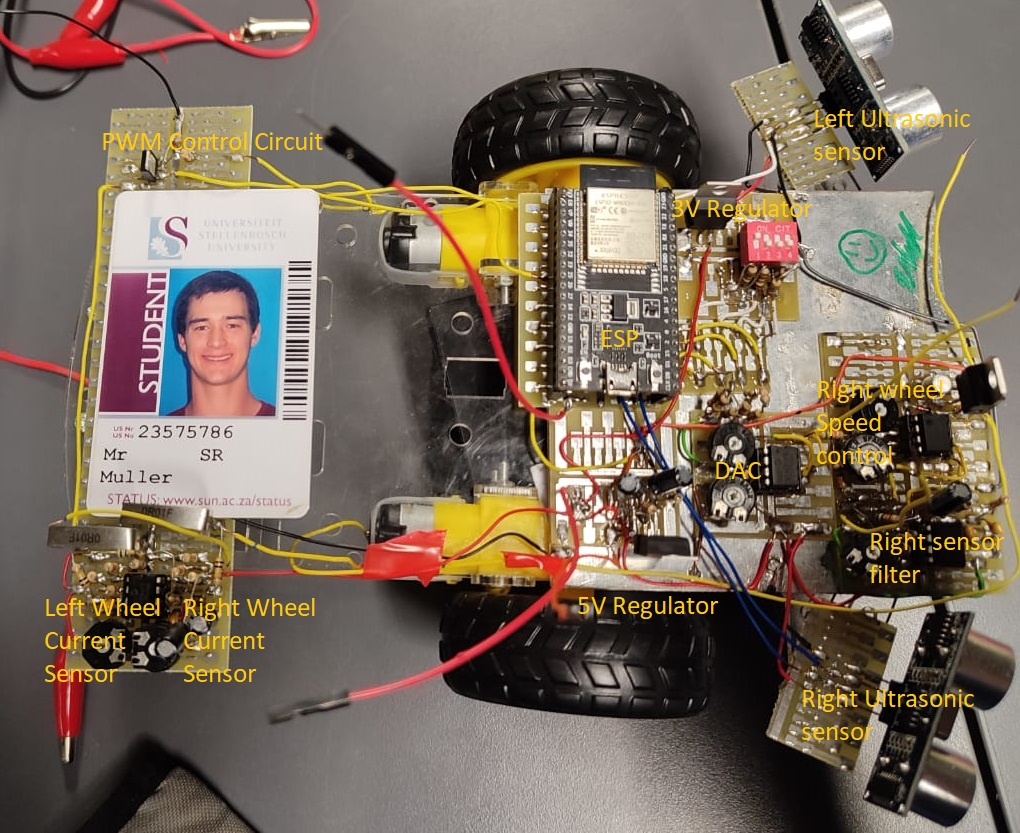
\includegraphics[width = 0.8\textwidth]{./Figures/FullCircuit_2.jpeg}
\caption{Labelled circuit of the current system}
\label{fig:full_prac_cir}
\end{figure}

\subsection{Circuit}
\begin{figure}[H]
\centering
\includegraphics[width = 0.4\textwidth]{./Figures/Cursens_Cir_Left_Card.jpeg}
\caption{Labelled circuit of current sensor and PWM control circuit.}
\label{fig:cursen_cir_card}
\end{figure}
